\label{chap:benchTopMeas}

Due to the sensitivity of the beam coupling impedance to the boundary conditions of the equipment used, it is necessary to utilise different measurement techniques to fully analyse the impedance of accelerator structures.

\section{Low Q-factor Impedances}
\label{sec:coax_wire_meth}

For structures that are expected to contain mostly low Q-resonances (i.e. resistive wall impedance) it is appropriate to use the coaxial wire method \cite{Gluckstern:WireMeasImp, Vaccaro:ImprovedWireMeth}, sometimes also called the stretched wire method. This method relies on the similarity of the electromagetic field profile due to an ultrarelativistic charged particle and that of a short electrical pulse sent along a coaxial wire. 

A moving charged particle produces an electromagnetic field in an arc transverse to its direction of motion, where the angle of the arc opening is inversely proportional to the relativistic factor of the particle $\gamma$. For an ultrarelativistic particle ($\gamma \rightarrow \infty$), the field becomes entirely perpendicular to the direction of motion. If we place a conductive wire along the same path we would expect the charged particle to take (in most cases this is well represented by a straight wire), a short electrical pulse sent along this wire would propogate in the TEM (Transverse Electrical and Magnetic field) mode, producing a field profile similar to that emitted by the ultrarelativistic charged particle (see. Fig. \ref{fig:coax-part-profile})


\begin{figure}
\begin{center}
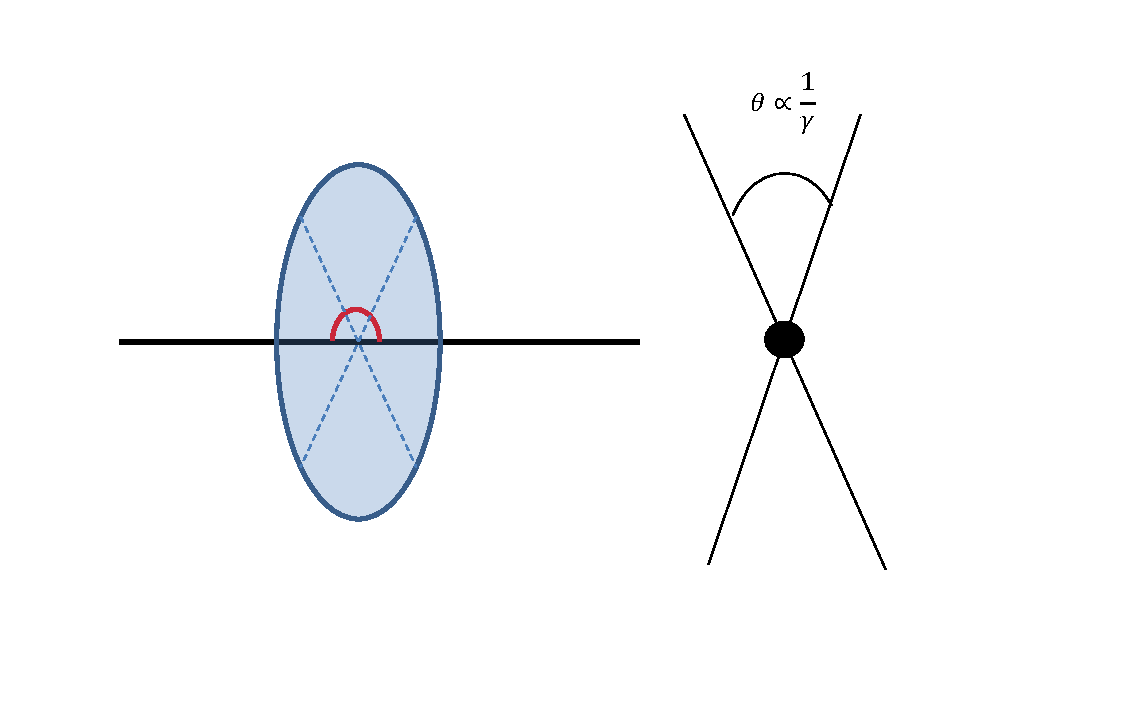
\includegraphics[width=0.6\textwidth]{Bench_Top_Measurements/figures/coaxial-particle-fields.pdf}
\end{center}
\caption{Comparison of the electromagnetic field profile of a moving charged particle and a short time pulse propagating along a coaxial wire.}
\label{fig:coax-part-profile}
\end{figure}

\subsection{Classical Coaxial Wire Method}

The classical coaxial wire method, first proposed in it's present form by V. Vaccarro in 1990 \cite{Vaccaro:ImprovedWireMeth}, is a transmission method that measures the complex transmission coefficient of a DUT (Device Under Test) made up of the equipment whose impedance is to be measured and a coaxial wire passing through it. 

The experimental setup is as shown in Fig. \ref{fig:classic-coax}. Firstly the external circuit (i.e. everything which is not the DUT such as VNA, cables, transition between connections etc.) is matched to the characteristic impedance of the coaxial line inside the DUT. This is done by measuring the reflection coefficient $\Gamma$ for the setup with only one port connected to the DUT and the other end terminated by an open connection. Knowing the characteristic impedance of the VNA and associated cables (typically $Z_{c0} = 50\Omega$), we can easily calculate the characteristic impedance of the DUT, $Z_{c}$, from the relation,

\begin{equation}
\Gamma = \frac{Z_{c} - Z_{c0}}{Z_{c} + Z_{c0}}.
\end{equation}

It is then possible to electrically match the characteristic impedance by adding a resistive network between the DUT and the external circuit. This may be done in two ways:

\begin{enumerate}
\item{Adding resistors in series just before the DUT to resistively match the characteristic impedance (as seen by the DUT) of the VNA and associated measurement setup to that of the DUT, such that the series resistance $R_{s}=Z_{c0}-Z_{0}$. Often an attenuator is used to reduce the effect of reflections from the mismatch between the VNA and the resistor, shown in Fig.~\ref{fig:resMatch}.}
\item{The use of two way matching, using a parallel ($R_{p}$) and series ($R_{s}$) resistor, as shown in Fig.~\ref{fig:twoWayMatch}. The values for these resistances are given by}
\begin{align}
R_{p} = Z_{c0}\frac{\sqrt{Z_{c0}}}{Z_{c0}-Z_{0}} \nonumber \\
R_{s} = Z_{c0} - \frac{Z_{c0}R_{p}}{Z_{c0}+R_{p}} \nonumber
\end{align}
\end{enumerate} 

\begin{figure}
\subfigure[]{
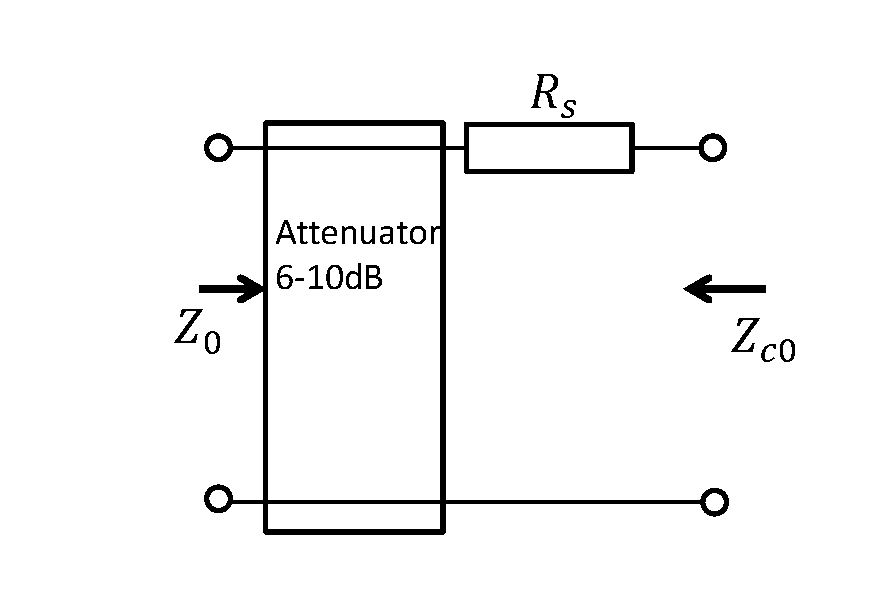
\includegraphics[width=0.45\textwidth]{Bench_Top_Measurements/figures/matching1Way.pdf}
\label{fig:resMatch}
}
\subfigure[]{
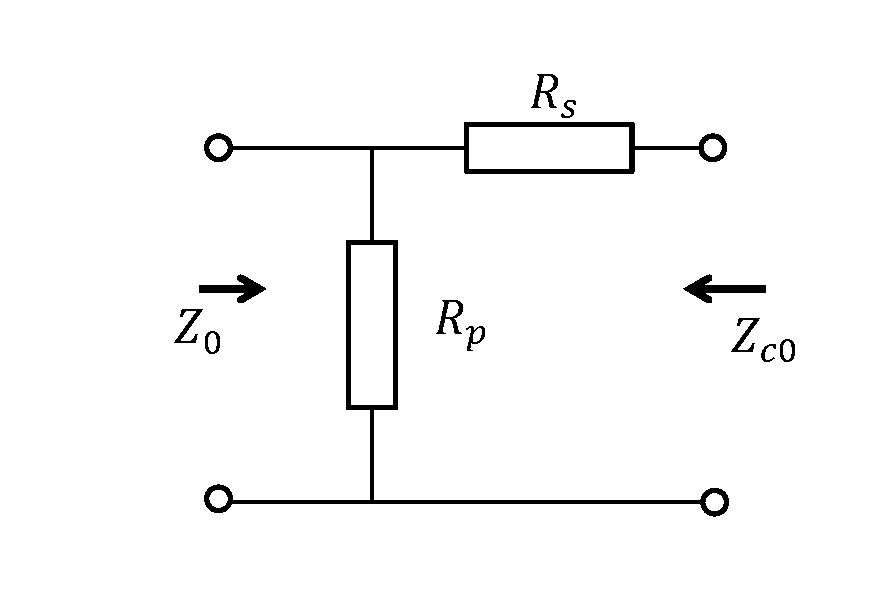
\includegraphics[width=0.45\textwidth]{Bench_Top_Measurements/figures/matching2Way.pdf}
\label{fig:twoWayMatch}
}
\caption{The resistive networks for matching a DUT to the attached measuring network (VNA and connecting cables). \subref{fig:resMatch} shows series resistive matching and \subref{fig:twoWayMatch} shows a two way matching network.}
\end{figure}

It is possible to use physical matching also using transition cones but these are costly, time consuming to construct, work only for a restricted frequency range and require new cones for each piece of equipment measured. And as can be seen in Fig. \ref{fig:matching-plot}, matching with a resistor is highly effective at removing the presence of reflections in coaxial measurements.

\begin{figure}
\begin{center}
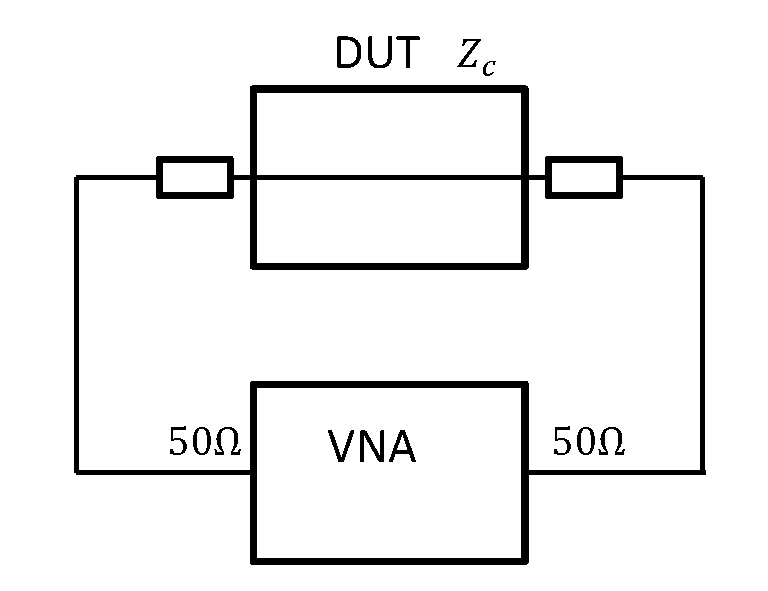
\includegraphics[width=0.6\textwidth]{Bench_Top_Measurements/figures/wire_meas_single_wire.pdf}
\end{center}
\caption{Experimental setup for a measurement of the beam coupling impedance using the classical coaxial wire method.}
\label{fig:classic-coax}
\end{figure} 

\begin{figure}
\begin{center}
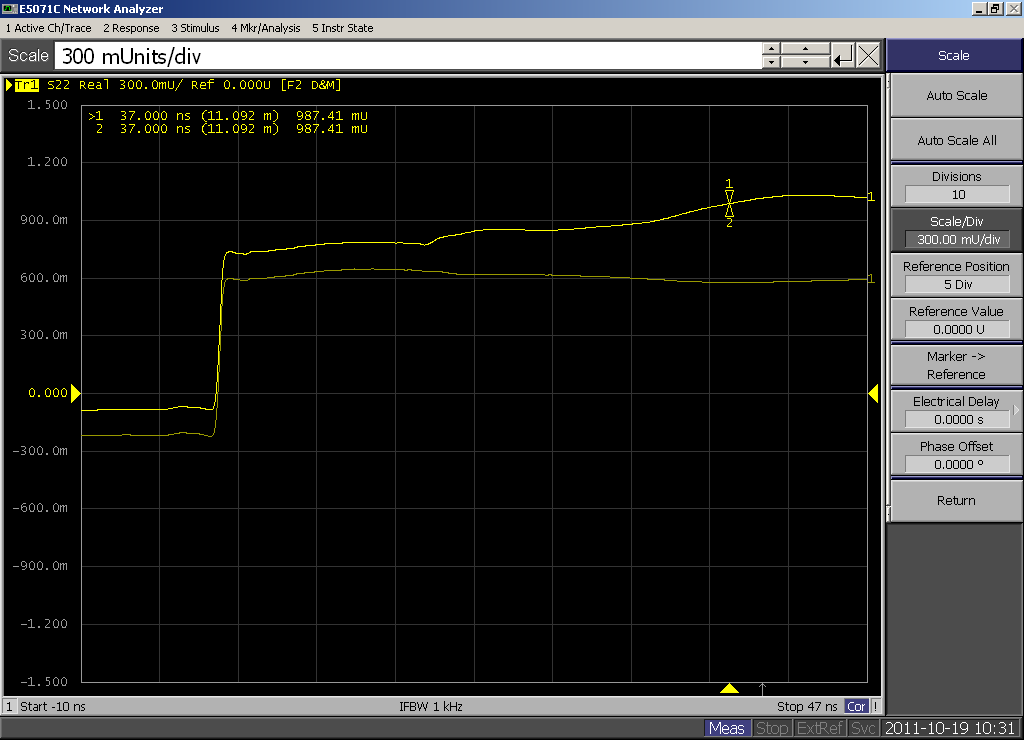
\includegraphics[width=0.6\textwidth]{Bench_Top_Measurements/figures/coax-matching-no-matching.png}
\end{center}
\caption{An example of a reflection measurement made with and without matching resistors. The faded line (lower trace) is the measurement with matching, the bold line (upper trace) that without. The reduction in the reflection can be seen due to the flatter line after the initial reflection.}
\label{fig:matching-plot}
\end{figure}

The values that we wish to measure to evaluate the beam coupling impedance of a device are the scattering parameters of the resulting circuit, in particular $S_{21}$, the normalised transmission parameter through the DUT. $S_{21}$ is calculated by taking the measured transmission parameter $S_{21,DUT}$ and dividing it by the transmission parameter through a reference line of the same physical length as the DUT,

\begin{equation}
S_{21} = \frac{S_{21,DUT}}{S_{21,REF}}.
\end{equation}

The effect of this is to correct the measured phase change in the DUT to be that only caused by the imaginary component of the beam coupling impedance.

There are subsequently a number of ways to evaluate the beam coupling impedance of the DUT depending on it's expected properties. For devices that are expected to have either a small impedance, or those that are physically very short in length, it is possible to use the so called lumped impedance formula \cite{Hahn:BenchMeasInter, Hahn:ValidityImpMeas};

\begin{equation}
Z = 2Z_{c} \frac{1-S_{21}}{S_{21}}.
\end{equation}

For distributed impedances, it is suitable to use the so called log formula (called so due to the exponential attenuation of the signal causing a log function to appear in the evaluation) \cite{Hahn:BenchMeasInter, Hahn:ValidityImpMeas, Jensen:ImprovLogForm},

\begin{equation}
Z = -2Z_{c} ln \left( S_{21} \right).
\end{equation}

For long components or measurements at very high frequencies there exists the improved log formula. This takes into account more completely the electrical length of the device, given by

\begin{equation}
Z = -2Z_{c} ln \left( S_{21}  \right) \left( 1 + j\frac{ln \left( S_{21}\right) }{2\Theta}  \right)
\end{equation}

where $\Theta = 2\pi \frac{L}{\lambda}$ is the normalised electrical length of the device, $L$ the length of the device. It is possible to see that the lumped impedance formula can be used when $\Theta \leq 1$, and the improved log formula becomes useful for $\Theta \geq 5$ \cite{Jensen:ImprovLogForm}.




\subsection{Resonator Coaxial Wire Method}
\label{sec:reson-coax-meth}

An alternative method for measuring the beam coupling impedance is by using the so called resonator method. The setup for this method is similar to that of the classical coaxial wire method, except that the matching resistor network between the VNA and DUT is replaced by a weak capacitive coupling ($S_{11} < 0.5dB$, remembering that $0dB$ means full reflection, i.e. no coupling) at both ends of the DUT. This then produces a structure which resonates at frequencies where the wavelength corresponds to the classical closed structure form,

\begin{equation}
\lambda = \frac{2L}{n}
\end{equation}

where $\lambda$ is the wavelength of the resonance, $n$ the harmonic of the resonance and $L$ the length of the device. 

The resonant method enables accurate measurement of the transmission losses due to the real longitudinal impedance. Additional advantages are that no matching is required, and a large number of mechanical uncertainties (electrical connections, consistency of calibration) can be avoided. However it can be seen that the frequency resolution is limited due to the length of the DUT so the method is not recommended as the only measurement method for structures expected to contain high-Q, narrowband resonances. It can however be used to corroborate the results obtained using the classical method.

For each resonant peak, the loaded Q-factor and the frequency of the resonance are measured. For a weak coupling at both ends of the DUT, we can write the coupling coefficient $k$ as

\begin{equation}
k = \frac{\left| S_{21} \right|}{1 - \left| S_{21} \right| }.
\label{eqn:coupling_coeff}
\end{equation}

The difference between the unloaded $Q$-factor, $Q_{0}$ , and the loaded $Q$-factor, $Q_{L}$, is a function of $k$. The loaded Q is the Q of the DUT resonance coupled with the measurement circuitry, and the unloaded Q the Q of the DUT resonance in isolation. We can get an approximate correction by using the formula

\begin{equation}
Q_{0} = Q_{L} \left( 1 + k  \right).
\label{eqn:Q_correc}
\end{equation}

Subsequently the measured line attenuation (in Np/m) is then calculated

\begin{equation}
\alpha_{m} = \frac{\pi}{\lambda Q_{0}}.
\label{eqn:atten}
\end{equation}

Note that this attenuation includes both that from the beam coupling impedance as well as that due to the finite resistance of the wire material. We can estimate the attenuation due to the wire material as

\begin{equation}
\alpha_{w} = \sqrt{\pi \rho_{w} \epsilon f} \frac{1}{d ln D/d}
\label{eqn:wire_atten}
\end{equation}

where $\rho_{w}$ is the wire resistivity, $\epsilon$ the wire permitivitty, $f$ the frequency, $d$ the diameter of the inner conductor and $D$ the diameter of the outer conductor (typically the vacuum beam pipe diameter). At very low frequencies the finite skin depth of the inner conductor would also have to be taken into account. Using the corrected attentuation $\alpha = \alpha_{m} - \alpha_{w}$, the real longitudinal impedance per unit length can be found to be 

\begin{equation}
\Re e\left\{ Z \right\} = 2Z_{c} \alpha
\label{eqn:res_imp}
\end{equation}

\begin{figure}
\begin{center}
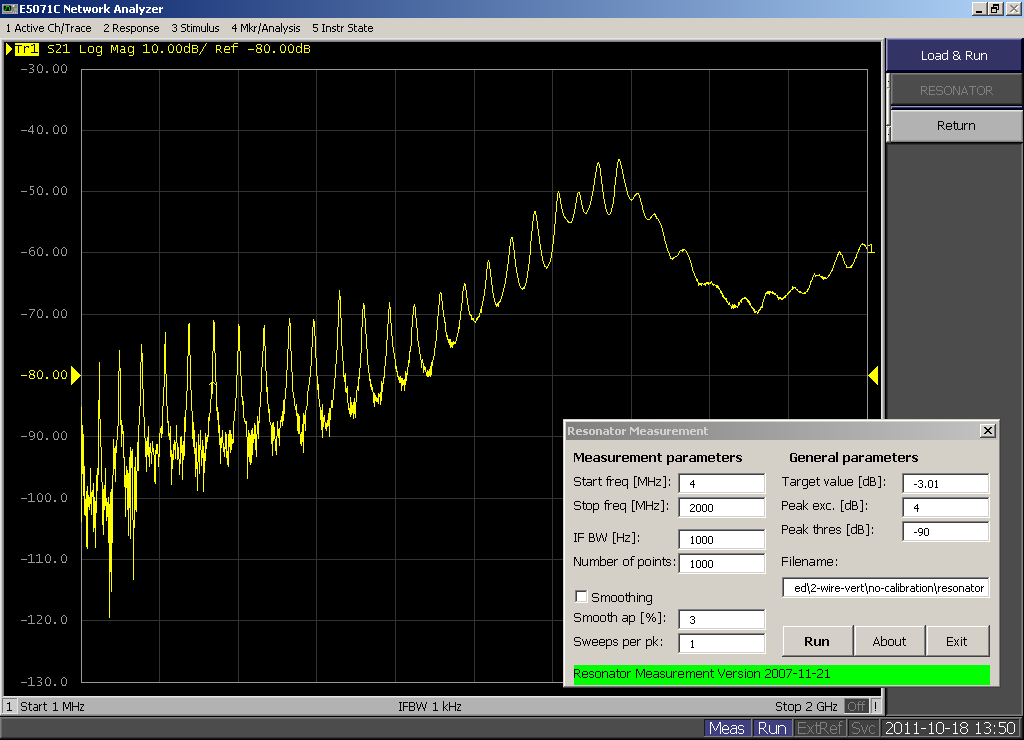
\includegraphics[width=0.6\textwidth]{Bench_Top_Measurements/figures/coax-resonator.png}
\end{center}
\caption{An example of the resonance pattern seen whilst performing measurements using the resonant method. Each peak corresponds to one data point in the final measurements. Taken from measurements of the LHC injection kicker magnets.}
\label{fig:res-resonancce-examples}
\end{figure}

It is more involved to calculate the imaginary impedance using the resonant method. In particular it is necessary to calculate the resonant frequencies of a pipe open at both ends of the same length of the DUT made of a good conducting material (i.e. the physical length is equal to the electrical length). This allows the comparison to the measured resonant frequencies of the DUT, the difference between which is dependent on the imaginary impedance.

Considering the complex impedance of the two measurements, $Z_{DUT}$ for the DUT and $Z_{REF}$ for a perfectly conducting reference pipe, they can be written as

\begin{align}
Z_{DUT} & =  R + jX_{1}  =  Z_{1}e^{j \phi} \\
Z_{REF} & =  jX_{2}  =  Z_{2}e^{j.0}
\end{align}

where $R$ is the resistive component of the DUT impedance, $X_{1/2}$ the imaginary component of the impedance (DUT and reference pipe respectively), $\phi$ is the angle of DUT impedance projected onto a complex plane and $Z_{2} = \sqrt{R^{2} + X^{2}}$. If we consider a measured value depedent on the impedance, for example the transmission parameter $S_{21}$ at a resonant peak, we have the following relations

\begin{align}
S_{21}^{DUT} = S_{0}e^{j \left( \omega_{1}t + \phi \right)} \\
S_{21}^{REF} = S_{0}e^{k \left( \omega_{2}t \right)}
\end{align}

where $S_{0}$ is some normalised scalar, $\omega_{1/2}$ is the frequency of the resonance and $t = \frac{L}{c}$ . Thus for a pair of corresponding peaks from resonance measurements for which we have measured $\omega_{1}$ and $\omega_{2}$ we can equate $S_{21}^{DUT} = S_{21}^{REF}$ and thus show

\begin{equation}
\phi = t \left( \omega_{2} - \omega_{1} \right).
\end{equation}

Subsequently we can see that

\begin{equation}
X = Z_{DUT} sin \phi = R \frac {sin \phi}{cos \phi} = R tan \phi
\end{equation}

where $R = \Re e(Z)$.

\subsection{Transverse Impedance Measurements}

The above methods give a general impression of how to carry out coaxial wire measurements of the impedance of accelerator components. Directly applied as described they allow the measurement of the longitudinal impedance of a DUT. However, from a beam stability point of view, it is also interesting to look at the transverse impedance of a device. In particular it would be useful to have a method of determining the vertical/horizontal dipolar (or driving) impedance and the vertical/horizontal quadrupolar (detuning) impedance of any device. In this section we describe how to do this for structures with top/bottom, left/right symmetry and then generalise to asymmetric structures, with illustration from simple examples evaluated using simulations.

To allow a complete explanation of how to verify the methods of measuring transverse impedances, let us first consider the general form of the $m$-th order ($m = 0, 1, 2,...$) longitudinal beam coupling impedance, given by \cite{Chao:PhysColEff, Tsutsui:OnSingleWire}

\begin{equation}
\bar{Z}_{m} = \frac{-1}{I^{2}} \int dV \mathbf{\bar{E}_{m}. \bar{J}_{m}^{*}}
\end{equation}

where $\bar{J}_{m}$ is the current density of the source. For a beam propogating along the z-axis with an offset $a$ and moment $cos \left( m \theta \right)$,

\begin{equation}
\mathbf{\bar{J}_{m}} = \frac{I}{\pi a^{m +1} \left( 1 + \delta_{m0} \right)} \delta \left( r - a \right) cos \left( m \theta \right) exp \left( j \left( \omega t - k z  \right) \right) \mathbf{e_{z}}.
\end{equation}

The electromagnetic field associated with a given current source $\mathbf{\bar{J}_{m}}$ is $\left( \mathbf{\bar{E}_{m}}, \mathbf{\bar{H}_{m}} \right)$. 

It can be seen that any different azimuthal components of the $m$-th field of order $n$ (i.e. $sin \left( n\theta \right)$ and $cos \left( n\theta \right)$ terms) are neglected in this treatment. To allow the treatment of coupling between different azimuthal orders we can define a longitudinal beam coupling impedance $Z_{m,n}$ (where $m,n = 0, \pm 1, \pm 2, ... $)

\begin{equation}
Z_{m,n} = \frac{-1}{I^{2}} \int dV \mathbf{E_{m}. J_{n}^{*}}
\end{equation}

where

\begin{equation}
\mathbf{J_{m}} = \frac{I}{2 \pi a^{|m |+1}} \delta \left( r - a \right) exp \left(j m \theta \right) exp \left( j \left( \omega t - k z  \right) \right) \mathbf{e_{z}}.
\end{equation}

Importantly, this allows us to see that 

\begin{align}
\mathbf{\bar{J}_{0}} &= \mathbf{J_{0}} \nonumber \\
\mathbf{\bar{J}_{m}} &= \mathbf{J_{m}} + \mathbf{J_{-m}}.
\end{align}

From here we use the principle of superposition for electromagnetic fields (i.e. we neglect any non-linearities of the surrounding materials), and thus can derive

\begin{align}
\bar{Z}_{0} &= Z_{0} \\
\bar{Z}_{x} &= \bar{Z}_{1} = Z_{1,1} + Z_{1,-1} + Z_{-1,1} + Z_{-1,-1} = kZ^{dip}_{x}\\
\bar{Z}_{x} &= \bar{Z}_{1} \text{(cos replaced with sin)}= Z_{1,1} - Z_{1,-1} - Z_{-1,1} + Z_{-1,-1} = kZ^{dip}_{y}\\
\bar{Z}_{m} &= Z_{m,m} + Z_{m,-m} + Z_{-m,m} + Z_{-m,-m}, m=1,2,...
\end{align}

From this start we will apply this to both two wire measurements and to displaced single wire measurements.

\subsubsection{Two Wire Measurements}

It is possible to directly measure the dipolar impedance of a device through the use of a two wire coaxial method. The measurement setup is identical to that of the single wire method, except that two wires, seperated by distance $\Delta$, are placed in the device, and a 180$^{\circ}$ hybrid is place between the wires and the VNA at both ends of the device. This setup is illustrated in Fig. \ref{fig:two_wire_measure}

\begin{figure}
\begin{center}
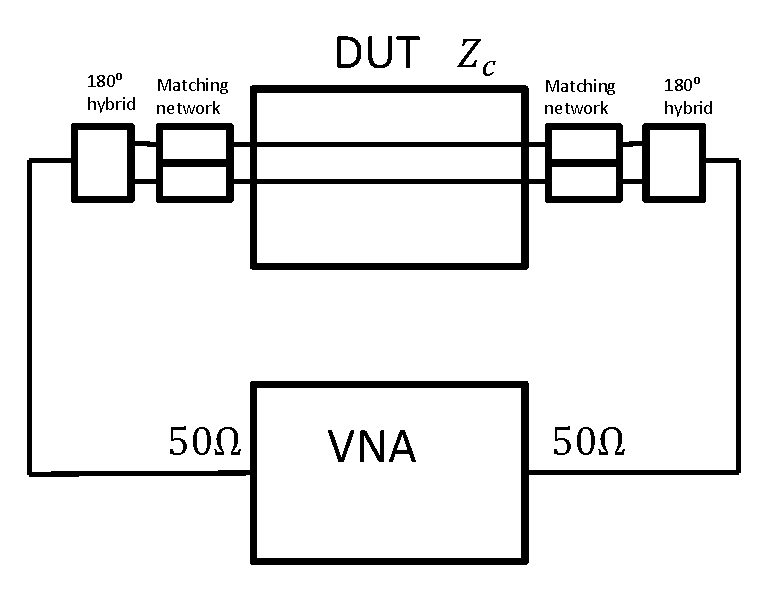
\includegraphics[width=0.6\textwidth]{Bench_Top_Measurements/figures/wire_meas_two_wire.pdf}
\end{center}
\caption{Measurement setup for measurements of the dipolar beam coupling impedance using the two wire setup for the classical coaxial wire method.}
\label{fig:two_wire_measure}
\end{figure}

The measurements are done in the same way as described in the previous sections for either the classical transmission method or the resonator method. When using the classical coaxial wire method, both wires are individually matched to $Z_{c0}$. By using two wires each carrying a signal 180$^{o}$ out of phase with one another we produce a field pattern similar to a dipole and thus measure the dipole impedance in either the horizontal or vertical plane depending on the orientation of the two wires. 

What is directly measured is the longitudinal impedance of just the dipole impedance, as is to be expected from the Panofsky-Wenzel theorem (see Sec.~\ref{sec:PanWen} for further explanation). 

For two wire placed at positions $x = \pm a$ relative to the centre of the aperture, the source current density is given by \cite{Tsutsui:OnSingleWire}

\begin{align}
J & =  I \left( \delta \left( x - a \right) - \delta \left( x + a  \right) \right) \delta (y) exp \left( j \left( \omega t - kz \right) \right) \nonumber \\
& =  \frac{I}{\pi a} \displaystyle\sum\limits_{m=-\infty}^{\infty} exp \left(j \left( 2m +1 \right) \theta \right) exp \left( j \left( \omega t - kz \right) \right) \nonumber \\
& =  2\displaystyle\sum\limits_{m=-\infty}^{\infty} a^{|2m + 1 |} J_{2m + 1}.
\end{align}

The impedance is then

\begin{align}
Z & =  - \frac{1}{I^{2}} \int dV \left( 2\displaystyle\sum\limits_{m=-\infty}^{\infty} a^{|2m + 1 |} E_{2m + 1}  \right)  \left( 2\displaystyle\sum\limits_{n=-\infty}^{\infty} a^{|2n + 1 |} J_{2n + 1}^{*}  \right) \nonumber \\
& =  4 \displaystyle\sum\limits_{m,n} a^{|2m + 1 | + |2n + 1|} Z_{2m + 1, 2n+1} \nonumber \\
& =  \left(2a \right)^{2}\left( Z_{1,1} + Z_{-1,1} + Z_{1,-1} + Z_{-1,-1} \right) + O(a^{4}) \nonumber \\
& =  (2a)^{2}\bar{Z}_{x} + O(a^{4}). 
\end{align}

Again using the Panofsky-Wenzel theorem we can deduce that the transverse dipolar impedance $Z^{dip}_{x/y}$ is given by 

\begin{equation}
Z^{dip}_{x/y} = \frac{\bar{Z}_{x/y}}{k} = \frac{c}{\omega} \frac{Z}{\Delta^{2}}
\end{equation}

where $\Delta = 2a$ and $Z$ is the measured complex impedance.

\subsubsection{Structures with Top/Bottom, Left/Right Symmetry}

If we consider a source particle at $x_{1} = a_{1}cos\theta_{1}, y_{1} = a_{1}sin\theta_{1}$ and a test particle at $x_{2} = a_{2}cos\theta_{2}, y_{2} = a_{2}sin\theta_{2}$, the source current density is

\begin{align}
J_{z} &= I\delta \left( x-x_{1} \right) \delta \left( y-y_{1} \right) exp \left( k \left( \omega t - kz \right) \right) \nonumber \\
          &=\displaystyle\sum\limits_{m=-\infty}^{\infty}a_{1}^{|m|}exp\left( -jm\theta_{1} \right) J_{m}
\end{align}

The impedance would therefore be

\begin{align}
Z = &\frac{-1}{I^{2}} \int dV \left( \displaystyle\sum\limits^{\infty}_{m=-\infty} a_{1}^{|m|} exp \left( jm\theta_{1} \right) E_{m}\right) \left( \displaystyle\sum\limits^{\infty}_{n=-\infty} a_{1}^{|n|} exp \left( jn\theta_{2} \right) J^{*}_{n}\right) \nonumber \\
   = &\displaystyle\sum\limits^{\infty}_{m,n=-\infty} a_{1}^{|m|} a_{2}^{|n|} exp\left( -jm\theta_{1} \right) exp\left( -jn\theta_{2} \right) Z_{m,n} \nonumber \\
   = &Z_{0,0} + \left( x_{1}- jy_{1} \right)Z_{1,0} + \left( x_{1} + jy_{1} \right)Z_{-1,0} + \left( x_{2} + jy_{2} \right)Z_{0,1} +  \left( x_{2} - jy_{2} \right)Z_{0,-1} \nonumber \\
      & +\left( x_{1} - jy_{1} \right)^{2}Z_{2,0} +  \left( x_{1} - jy_{1} \right)\left( x_{2} - jy_{2} \right)Z_{1,-1} + \left( x_{2} - jy_{2} \right) Z_{0,-2} \nonumber \\
      & +\left( x_{1} - jy_{1} \right)\left( x_{2} + jy_{2} \right)Z_{1,1} + \left( x_{1} + jy_{1} \right) \left( x_{2} - jy_{2} \right) Z_{-1,-1} \nonumber \\
      & +\left( x_{1} + jy_{1} \right)^{2}Z_{-2,0} + \left( x_{1} + jy_{1} \right)\left( x_{2} - jy_{2} \right) Z_{-1,1} + \left( x_{2} - jy_{2} \right)^{2}Z_{0,2} \nonumber \\
      & +O\left( \left(  x_{1},y_{1},x_{2},y_{2} \right)^{3} \right).
\label{eqn:gen_imp}
\end{align}

By applying Panofsky-Wenzel we see that

\begin{align}
kZ_{x} =\frac{\partial Z}{\partial x_{2}} = & Z_{0,1} + Z_{0,-1} + \left( x_{1} - jy_{1} \right) Z_{1,-1} + 2\left( x_{2} - jy_{2} \right) Z_{0,-2} \nonumber \\
						&+ \left( x_{1} - jy_{1} \right) Z_{1,1} + \left( x_{1} + jy_{1} \right) Z_{-1,-1} + \left( x_{1} + jy_{1} \right) Z_{-1,1} + 2\left( x_{2} + jy_{2} \right) Z_{0,2} \nonumber \\
						& + O\left( \left( x_{1},y_{1},x_{2},y_{2} \right)^{2} \right) \nonumber \\
						= & Z_{0,1} + Z_{0,-1} + x_{1}\bar{Z}_{x} + jy_{1} \left( -Z_{1,-1} - Z_{1,1} + Z_{-1,-1} + Z_{-1,1} \right) \nonumber \\
						& + x_{2}\left( 2Z_{0,-2} + 2Z_{0,2}  \right) + jy_{2}\left( -2Z_{0,-2} + 2Z_{0,2}  \right) +  O\left( \left( x_{1},y_{1},x_{2},y_{2} \right)^{2} \right)
\end{align}

\begin{align}
kZ_{y} =\frac{\partial Z}{\partial y_{2}} = & jZ_{0,1} - jZ_{0,-1} - j\left( x_{1} - jy_{1} \right) Z_{1,-1} - 2j\left( x_{2} - jy_{2} \right) Z_{0,-2} \nonumber \\
						&+ j\left( x_{1} - jy_{1} \right) Z_{1,1} - j\left( x_{1} + jy_{1} \right) Z_{-1,-1} + j\left( x_{1} + jy_{1} \right) Z_{-1,1} + 2j\left( x_{2} + jy_{2} \right) Z_{0,2} \nonumber \\
						& + O\left( \left( x_{1},y_{1},x_{2},y_{2} \right)^{2} \right) \nonumber \\
						= & j\left(Z_{0,1} - Z_{0,-1} \right)+ y_{1}\bar{Z}_{y} + jx_{1} \left( -Z_{1,-1} + Z_{1,1} + Z_{-1,-1} + Z_{-1,1} \right) \nonumber \\
						& + y_{2}\left(- 2Z_{0,-2} - 2Z_{0,2}  \right) + jx_{2}\left( -2Z_{0,-2} + 2Z_{0,2}  \right) +  O\left( \left( x_{1},y_{1},x_{2},y_{2} \right)^{2} \right).
\end{align}

Two properties to note for later use are that

\begin{align}
\textbf{J}_{-m} \left( \omega \right) & = \textbf{J}_{m}^{*} \left( -\omega \right) \\
Z_{-m,-n} \left( \omega \right) & = Z_{m,n}^{*} \left( -\omega \right).
\end{align}

If we now assume a single wire rather than a source and test particle, such that $x_{1}=x_{2}=x_{0}, y_{1}=y_{2}=y_{0}$. This gives a source current density

\begin{align}
J & = I \delta \left( x-x_{0} \right)\delta \left( y-y_{0} \right) exp\left( j \left(\omega t -kz \right)\right) \nonumber \\
  & = \frac{I}{2\pi a} \delta \left( r-a \right)\displaystyle\sum\limits_{m=-\infty}^{\infty} exp\left( jm \left( \theta -\theta_{0} \right) \right) exp\left( jm \left( \theta -\theta_{0} \right) \right) exp\left( j \left( \omega t - kz \right) \right) \nonumber \\
  & = \displaystyle\sum\limits_{m=-\infty}^{\infty} a^{|m|}exp\left( -jm\theta_{0} \right)J_{m}.
\end{align}

We can then define $x_{0}=acos\theta_{0}, y_{0}=asin\theta_{0}$. Entering this into Eqn. \ref{eqn:gen_imp} gives

\begin{align}
Z &=&Z_{0,0} +  \left( x_{0} - jy_{0} \right) Z_{1,0} + \left( x_{0} + jy_{0} \right)  Z_{-1,0} + \left( x_{0} + jy_{0} \right) Z_{0,1} \nonumber \\
   &   &+ \left( x_{0} - jy_{0} \right) Z_{0,-1} + \left( x_{0} - jy_{0} \right)^{2} Z_{2,0} + \left( x_{0} - jy_{0} \right)^{2} Z_{1,-1} + \left( x_{0} - jy_{0} \right) ^{2}Z_{0,-2} \nonumber \\
   &   &+\left( x_{0} - jy_{0} \right) \left( x_{0} + jy_{0} \right) Z_{1,1} + \left( x_{0} + jy_{0} \right)\left( x_{0} - jy_{0} \right) Z_{-1,-1} + \left( x_{0} + jy_{0} \right)^{2}Z_{-2,0} \nonumber \\
   &   &+\left( x_{0} + jy_{0} \right)^{2} Z_{-1,1} + \left( x_{0} + jy_{0} \right)^{2}Z_{0,2} + O\left( \left(x_{0},y_{0} \right)^{2} \right) \nonumber \\
   &=&Z_{0,0} + x_{0}\left( Z_{1,0}+Z_{-1,0}+Z_{0,1}+Z_{0,-1} \right) +jy_{0} \left( -Z_{-1,0} + Z_{-1,0} + Z_{0,1} - Z_{0,-1} \right) \nonumber \\
   &   &+x_{0}^{2} \left(  Z_{1,-1}+Z_{1,1}+Z_{-1,-1}+Z_{-1,1} + Z_{2,0} + Z_{0,-2} + Z_{0,2} + Z_{-2,0} \right) \nonumber \\
   &   &+y_{0}^{2} \left(  -Z_{1,-1}+Z_{1,1}+Z_{-1,-1}-Z_{-1,1} - Z_{2,0} - Z_{0,-2} - Z_{0,2} - Z_{-2,0} \right) \nonumber \\
   &   &+2jx_{0}y_{0}\left( -Z_{2,0} - Z_{0,-2} + Z_{-2,0} + Z_{0,2} + Z_{-1,1} - Z_{1,-1} \right) \nonumber \\
   &=&Z_{0,0} + x_{0}\left( Z_{1,0}+Z_{-1,0}+Z_{0,1}+Z_{0,-1} \right) +jy_{0} \left( -Z_{-1,0} + Z_{-1,0} + Z_{0,1} - Z_{0,-1} \right) \nonumber \\
   &   &+x_{0}^{2} \left( \bar{Z}_{x} + Z_{2,0} + Z_{0,-2} + Z_{0,2} + Z_{-2,0} \right) \nonumber \\
   &   &+y_{0}^{2} \left( \bar{Z}_{y} - Z_{2,0} - Z_{0,-2} - Z_{0,2} - Z_{-2,0} \right) \nonumber \\
   &   &+2jx_{0}y_{0}\left( -Z_{2,0} - Z_{0,-2} + Z_{-2,0} + Z_{0,2} + Z_{-1,1} - Z_{1,-1} \right).
\label{eqn:gen_single_wire}
\end{align}

It can then be seen that if measurements are made with $x_{0} = 0$ and taking different values of $y_{0}$ that one obtains data with a parabolic fit in the $y_{0}$ axis. By fitting a curve to this we obtain constant (equal to the longitudinal impedance), linear and quadratic terms. Doing the same for $y_{0}=0$ allows us to derive two quadratic terms

\begin{align}
Z^{\perp}_{x} & = \left( \bar{Z}_{x} + kZ_{quad} \right)\frac{1}{k} =  Z^{dip}_{x} + Z_{quad}\\
Z^{\perp}_{y} & = \left( \bar{Z}_{y} - kZ_{quad} \right)\frac{1}{k}= Z^{dip}_{y} - Z_{quad} \\
\end{align}

where $Z_{quad}=\frac{1}{k}\left( Z_{0,2}+Z_{2,0}+Z_{0,-2}+Z_{-2,0}  \right) = \frac{2}{k}\left( Z_{0,2}+Z_{0,-2}  \right)$ (shown in the case of 2D structures externally bounded by a perfectly conducting boundary in \cite{Tsutsui:OnSingleWire}), representing the impedance due to the displacement of the test particle in an accelerator. As we can measure $\bar{Z}_{x/y}$ independently using the two wire method we can thus indepedently measure $Z_{quad}$ using a displaced single wire scan in both the x- and y-planes.

It can also be seen that

\begin{align}
Z^{\perp}_{x} + Z^{\perp}_{y} = \frac{1}{k}\left( \bar{Z}_{x} + \bar{Z}_{y} \right) = Z^{dip}_{x} + Z^{dip}_{y}
\end{align}

where $\bar{Z}_{x/y}$ can be measured independently which gives a method of obtaining confidence in the wire measurements.

\subsubsection{Asymmetric Structures}

If Eqn. \ref{eqn:gen_single_wire} is transformed from $\left( x,y \right)$ coordinates to $\left( a, \theta \right)$, the result is

\begin{align}
Z &=Z_{0,0} +a\left[ cos\theta \left( Z_{-1,0} + Z_{0,1} \right) +jsin\theta \left( Z_{-1,0} + Z_{0,1} \right)  cos\theta \left( Z_{1,0} + Z_{0,-1} \right) - jsin\theta \left( Z_{1,0} + Z_{0,-1} \right)\right] \nonumber \\
   &+a^{2}\left[ cos^{2} \left( Z_{1,1} + Z_{-1,-1} \right) + sin^{2} \left( Z_{1,1} + Z_{-1,-1} \right)\right] \nonumber \\
   &+a^{2}\left[ cos^{2} \left( Z_{2,0} + Z_{0,-2} +Z_{1,-1} \right) +2jsin\theta cos\theta\left( Z_{2,0} + Z_{0,-2} +Z_{1,-1} \right) \right] \nonumber \\
   & - a^{2}\left[sin^{2} \left( Z_{2,0} + Z_{0,-2} +Z_{1,-1} \right)\right] \nonumber  \\
   &+ a^{2}\left[ cos^{2} \left( Z_{-2,0} + Z_{0,2} +Z_{-1,1} \right) +2jsin\theta cos\theta\left( Z_{-2,0} + Z_{0,2} +Z_{-1,1}  \right) \right] \nonumber \\
   &+ a^{2}\left[sin^{2} \left( Z_{-2,0} + Z_{0,2} +Z_{-1,1}  \right) \right].
\end{align}

Grouping terms by order of depedence on $a$ and $\theta$ this becomes
\begin{align}
Z   &=Z_{0,0} + a\left[ e^{-j\theta}\left( Z_{-1,0} + Z_{0,1} \right) +  e^{j\theta}\left( Z_{1,0} + Z_{-0,1} \right)\right] \nonumber \\
     &+a^{2}\left[ \left( Z_{1,1} + Z_{-1,-1} \right) + e^{-2j\theta} \left(  Z_{2,0} + Z_{0,-2} +Z_{1,-1} \right) + e^{2j\theta} \left( Z_{-2,0} + Z_{0,2} +Z_{-1,1} \right) \right] \nonumber \\
     &=A_{1} + ae^{-j\theta}A_{2} + ae^{-j\theta}A_{3}+ a^{2}e^{-2j\theta}A_{4} +a^{2}e^{2j\theta}A_{5} +  a^{2}A_{6}
\label{eqn:rot_gen}
\end{align}

where $A_{1} = Z_{0,0}$, $A_{2} = Z_{0,1}+Z_{-1,0}$, $A_{3} = Z_{0,-1}+Z_{1,0}$, $A_{4} = Z_{0,2}+Z_{-1,1}+Z_{-2,0}$, $A_{5} = Z_{2,0}+Z_{1,-1}+Z_{0,-2}$ and $A_{6}=Z_{1,1}+Z_{-1,-1}$. Taking the earlier definition of $Z_{quad}$ it can be deduced that

\begin{align}
Z_{quad} & = \left( A_{4}+A_{5}+A_{6} - \bar{Z}_{x} \right)\frac{1}{k} =\frac{ A_{4}+A_{5}+A_{6}}{k} - Z^{dip}_{x} \\  
	    & = \left( A_{4}+A_{5} - \frac{\bar{Z}_{x}- \bar{Z}_{y}}{2}\right)\frac{1}{k} =\frac{ A_{4}+A_{5}}{k} - \frac{Z^{dip}_{x}-Z^{dip}_{y} }{2}.
\end{align}

Consideration of Eqn. \ref{eqn:rot_gen} lets it be seen that

\begin{align}
 A_{4}+A_{5}+A_{6} & = \frac{Z\left( a,0 \right)+Z\left( a,\pi \right) - 2Z\left( 0,0 \right)}{2a^{2}} \\
 A_{4}+A_{5} & = \frac{Z\left( a,0 \right)+Z\left( a,\pi \right) - Z\left( a,\frac{\pi}{2} \right)-Z\left( a,\frac{3\pi}{2} \right)}{2a^{2}}.
\end{align}

The constant impedance can also be seen to be found by taking a linear fit of the longitudinal impedance of a wire displaced in either the $\theta = 0$ or $\theta = \pi / 2$ plane, and taking the linear term of the fit. 

\subsection{Measurements on Example Geometries}

In this section shall be presented a number of example analyses of coaxial wire measurements done on geometries exhibiting top/bottom, left/right symmetry and an asymmetric structure. This permits a step-by-step guide to analysis of the wire measurements, which may not be immediately clear from the mathematical introduction. These simulations are carried out using both Ansoft HFSS\cite{hfss} and Maxwell\cite{maxwell} using a driven modal solution. 

The simulations with HFSS are carried out in the following manner: for representing the single wire measurement the measurement system is simulated by placing waveguide ports at either end of the geometry with a conducting cylinder placed as the inner conductor of the coaxial system. The transmission parameters are then acquired as a result of the simulations. The wire may then be displaced as neccessary for the displaced single wire measurements. For two wire measurements a quarter geometry may be simulated, using a quarter geometry with a perfect H boundary in the plane of the wires, and a perfect E boundary between the wires to enforce the dipolar field pattern.

Maxwell is a frequency domain code optimised for low frequencies (less thans 10s of MHz). It does not permit the use of waveguide ports, however it does allow the definition of current segments with phase changes between them. By considering the current (either a single current segment to simulate a single wire, or two current carrying segments 180$^{\circ}$ out of phase for two wires) to be the equivalent of a beam current, and assuming the inclusion of the current carrying component is a negligible perturbation to the geometry, the real impedance can be found by summing the power loss in the system. This can be seen to be equivalent to the beam induced heating experienced by a beam interacting with an impedance.

This can be thought of by comparing the system to a homogenous transmission line. The power $P$ of a wave travelling along the line is given by \cite{Kroyer:lowFreqColImp}

\begin{equation}
P = P_{0}e^{-2\alpha z}
\end{equation}

where $P_{0}$ is the power at the beginning of the transmission line, $\alpha$ is the attenuation coefficient and $z$ the distance along the line. By differentiation it can be seen that

\begin{equation}
\alpha = -\frac{1}{2P} \frac{dP}{dz} \approx \frac{1}{2P} \frac{\delta P}{\delta z}
\end{equation}

where $\delta P$ is the power lost over the short distance $\delta z$. The transmission parameter of a line $S_{21}$ is given by

\begin{equation}
S_{21} = e^{-\alpha \delta z}.
\end{equation}

If the impedance is evaluated using the log formula ($Z = Z_{c}ln S_{21}$), it can be seen that the real impedance is subsequently given by

\begin{equation}
\Re{}e \left( Z \right) = Z_{c} \frac{2 \delta P}{P}.
\end{equation}

Assuming a peak current $I_{0}$ on the wire, $P = I_{0}^{2}Z_{c}/2$, which gives

\begin{equation}
\Re{}e \left( Z \right) = \frac{2 \delta P}{I_{0}^{2}}.
\end{equation}

To acquire the transverse impedance for two wire simulations it is simply neccesary to normalise by the wavenumber $k=\omega / c$ and the seperation of the wire $\Delta$ 

\begin{equation}
Z_{dip} = \frac{c}{\omega \Delta^{2}} \frac{2 \delta P}{I_{0}^{2}}.
\end{equation}

\subsubsection{Structure with Top/Bottom, Left/Rght Symmetry}

For the structure exhibiting top/bottom, left/right symmetry we use the Tsutsui model of two parallel plates as shown in Fig.~\ref{fig:tsutsui-model}. We use this due to the model allowing the prediction of the longitudinal, dipolar and quadrupolar impedances for a wide variety of materials and frequency ranges \cite{Tsutsui:ferrKickLong,Tsutsui:DipoleKicker, Salvant:QuadKicker}. For these simulations a short segment of a Tsutsui geometry is simulated using two different materials, in this case graphite, to represent a structure with a poor conductivity ($\sigma_{graphite} = 7 \times 10^{4} S m^{-1}$), and 4A4 ferrite, to represent a magnetically lossy material (in this case, $\epsilon_{r} = 10$, $\sigma_{4A4} = 10^{-6} S m^{-1}$ (a mild conductivity is applied to prevent static build up in ferrite components in accelerators), and $\mu_{r} = \mu^{'} + j \mu^{"}$, shown in Fig.~\ref{fig:4a4permeability}.). In both cases the following dimensions are used: $a=25mm$, $b=5mm$, $d=5mm$. A structure of 150mm in length is used to reduce numerical noise due to the small losses given by the short length of the simulated DUT.

\begin{figure}
\subfigure[]{
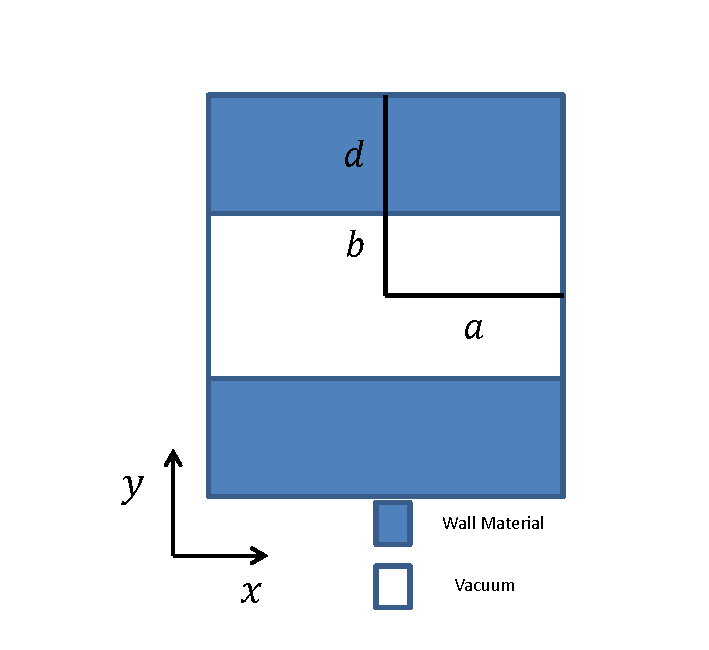
\includegraphics[width=0.45\textwidth]{Bench_Top_Measurements/figures/tsutsui-geometry.pdf}
\label{fig:tsutsui-model}
}
\subfigure[]{
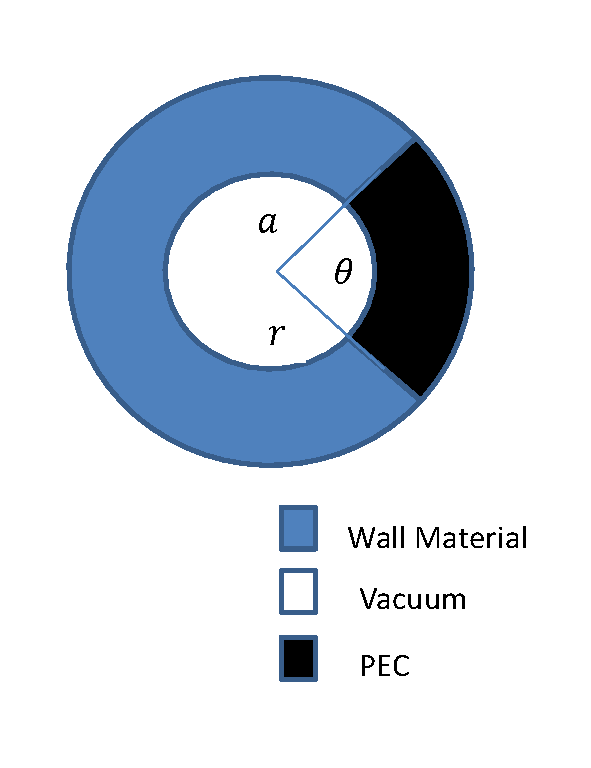
\includegraphics[width=0.45\textwidth]{Bench_Top_Measurements/figures/zannini-model-geo.pdf}
\label{fig:zannini-model}
}
\caption{The geometries used for coaxial wire measurement simulations. For the geometry with top/bottom, left/right symmetry we use the Tsutsui model (\subref{fig:tsutsui-model}) using two parallel plates. For the asymmetric structure we use the Zannini-model for a C-core ferrite kicker magnet (\subref{fig:zannini-model}), which generates a constant term and a noticeable asymmetric term.}
\label{fig:wire-measure-geometries}
\end{figure}

\begin{figure}
\begin{center}
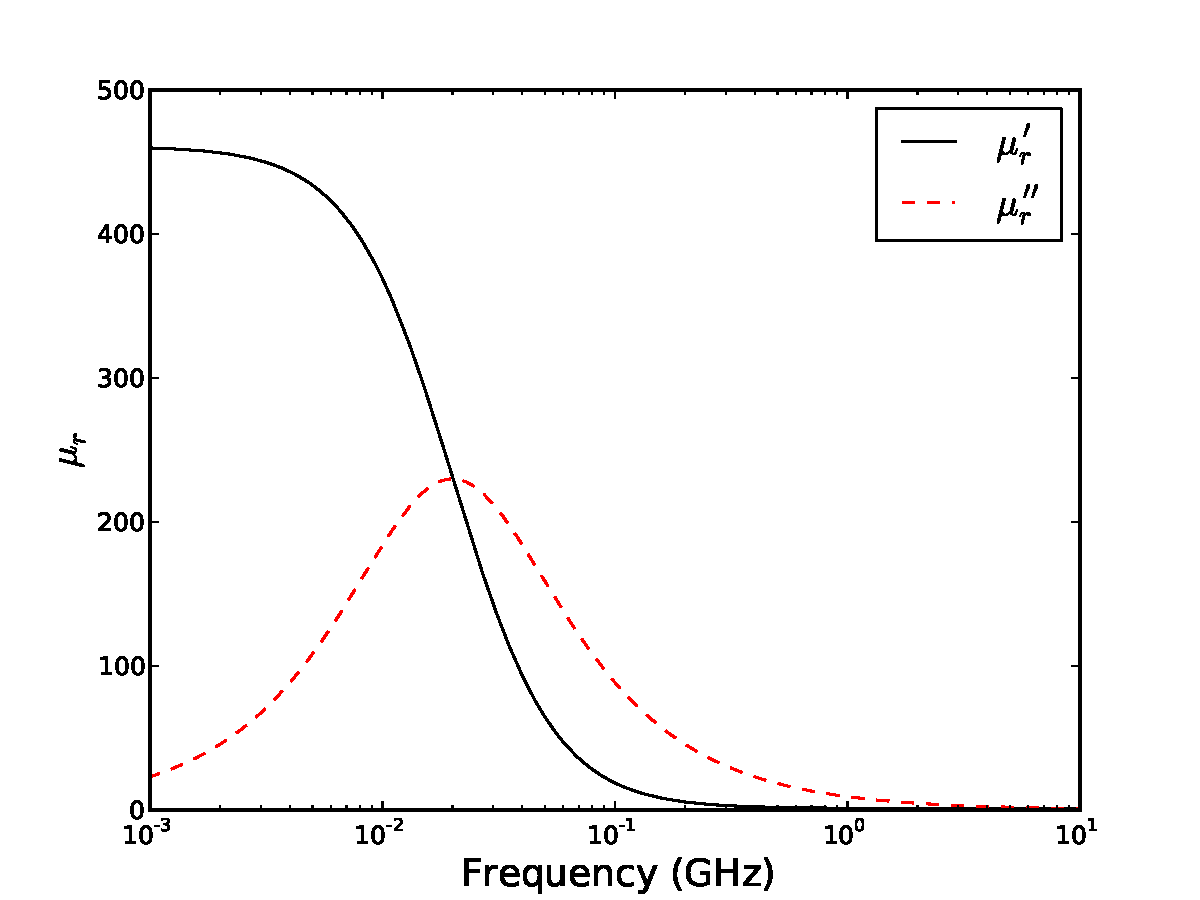
\includegraphics[width=0.45\textwidth]{Bench_Top_Measurements/figures/4A4FerrMu.pdf}
\end{center}
\caption{The complex permeability of 4A4 ferrite.}
\label{fig:4a4permeability}
\end{figure}

\begin{figure}
\begin{center}
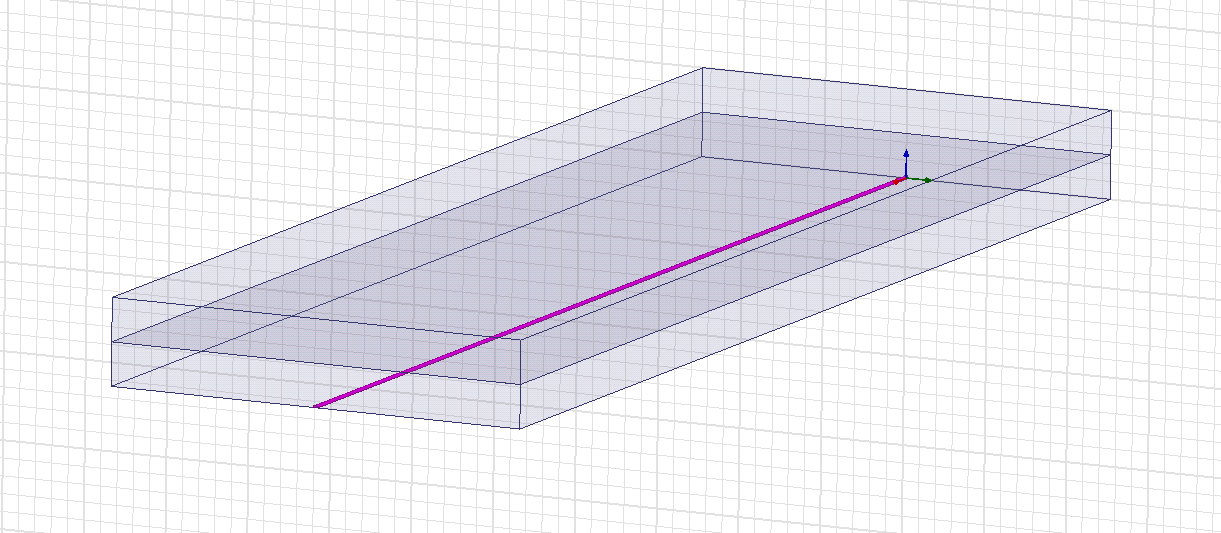
\includegraphics[width=0.5\textwidth]{Bench_Top_Measurements/figures/cross-section-coaxial-wire-measurements.png}
\end{center}
\caption{An example of the simulation model used for coaxial wire simulations. In this case a displaced single wire between two parallel plates. The wire is highlighted in purple.}
\label{fig:wire-sim-model}
\end{figure}

\subsubsection{Two Parallel Ferrite Plates}

For the simulations of two parallel ferrite plates the following parameters were used in HFSS; for the displaced single wire measurements a wire of 0.3mm in radius, and the following displacement used to acquire the total transverse terms:

\begin{enumerate}
\item{In the horizontal axis -  displaced between -6mm to +6mm at intervals of 2mm}
\item{In the vertical axis - displaced between -4mm to +4mm at intervals of 2mm.}
\end{enumerate}

For the two wire simulations, two wires of radius 0.3mm are used, with a seperation of 4mm in the x-dimension, and 3mm in the y-dimension. 4 simulation configurations are used described below:

\begin{enumerate}
\item{an adaptive mesh generation set to a convergence criterion of $S_{21}$ diverging by less than 0.005 between two subsequent solutions, at an adaptive frequency of 20MHz solving to a second order basis. A discrete frequency sweep is then carried out in the range 1-10MHz at 1MHz intervals.}
\item{an adaptive mesh generation set to a convergence criterion of $S_{21}$ diverging by less than 0.005 between two subsequent solutions, at an adaptive frequency of 200MHz solving to a second order basis. A discrete frequency sweep is then carried out in the range 10-100MHz at 10MHz intervals.}
\item{an adaptive mesh generation set to a convergence criterion of $S_{21}$ diverging by less than 0.005 between two subsequent solutions, at an adaptive frequency of 2GHz solving to a second order basis. A discrete frequency sweep is then carried out in the range 100MHz-1GHz at 100MHz intervals.}
\item{an adaptive mesh generation set to a convergence criterion of $S_{21}$ diverging by less than 0.005 between two subsequent solutions, at an adaptive frequency of 10GHz solving to a second order basis. A discrete frequency sweep is then carried out in the range 1-10GHz at 1GHz intervals.}
\end{enumerate}

These parameters are used to benefit from an appropriate mesh count for the given frequency range, thus increasing simulation speed by not using a high density mesh at frequencies where no benefits would be gained.

\begin{figure}
\subfigure[]{
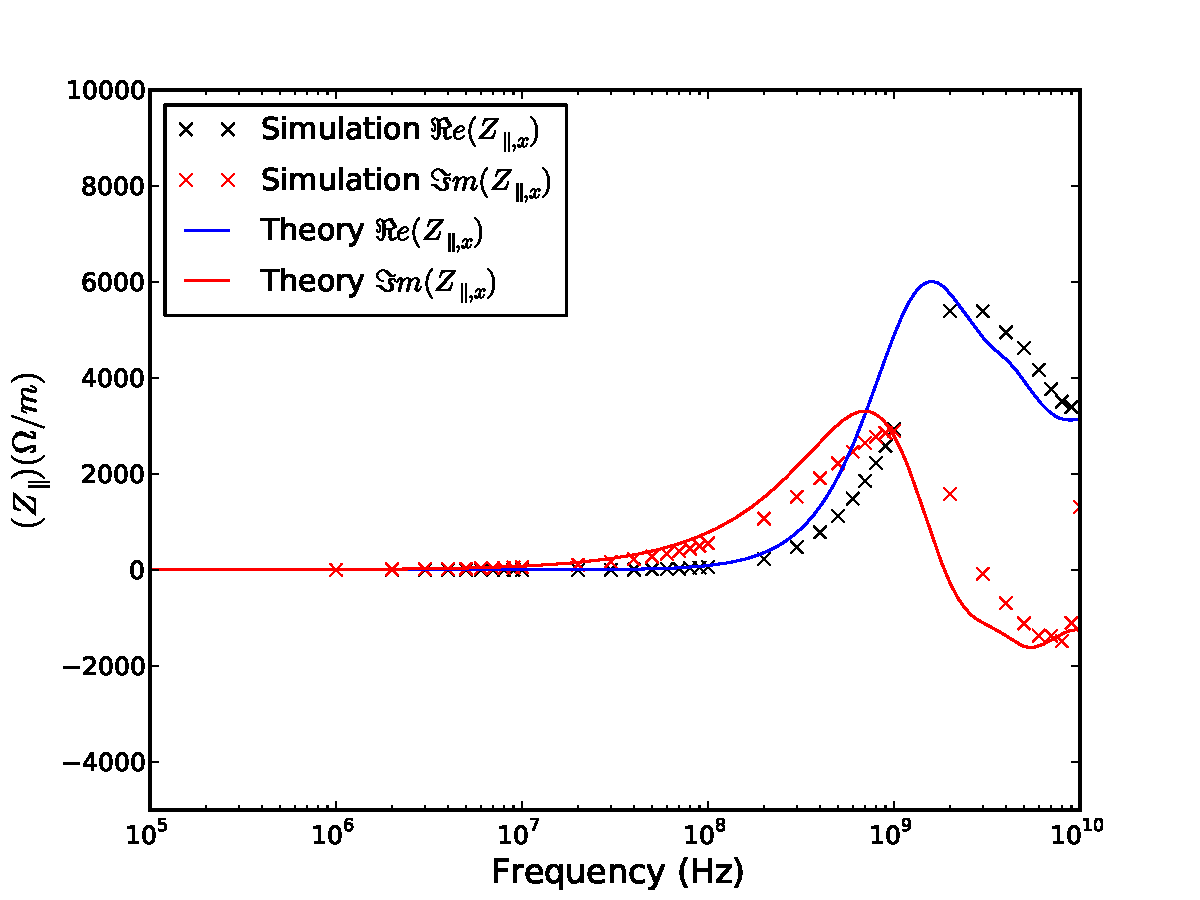
\includegraphics[width=0.5\textwidth]{Bench_Top_Measurements/figures/wire_meas/ferrite_plates/longitudinal-horizontal.pdf}
\label{fig:ferrite-plates-long-horz}
}
\subfigure[]{
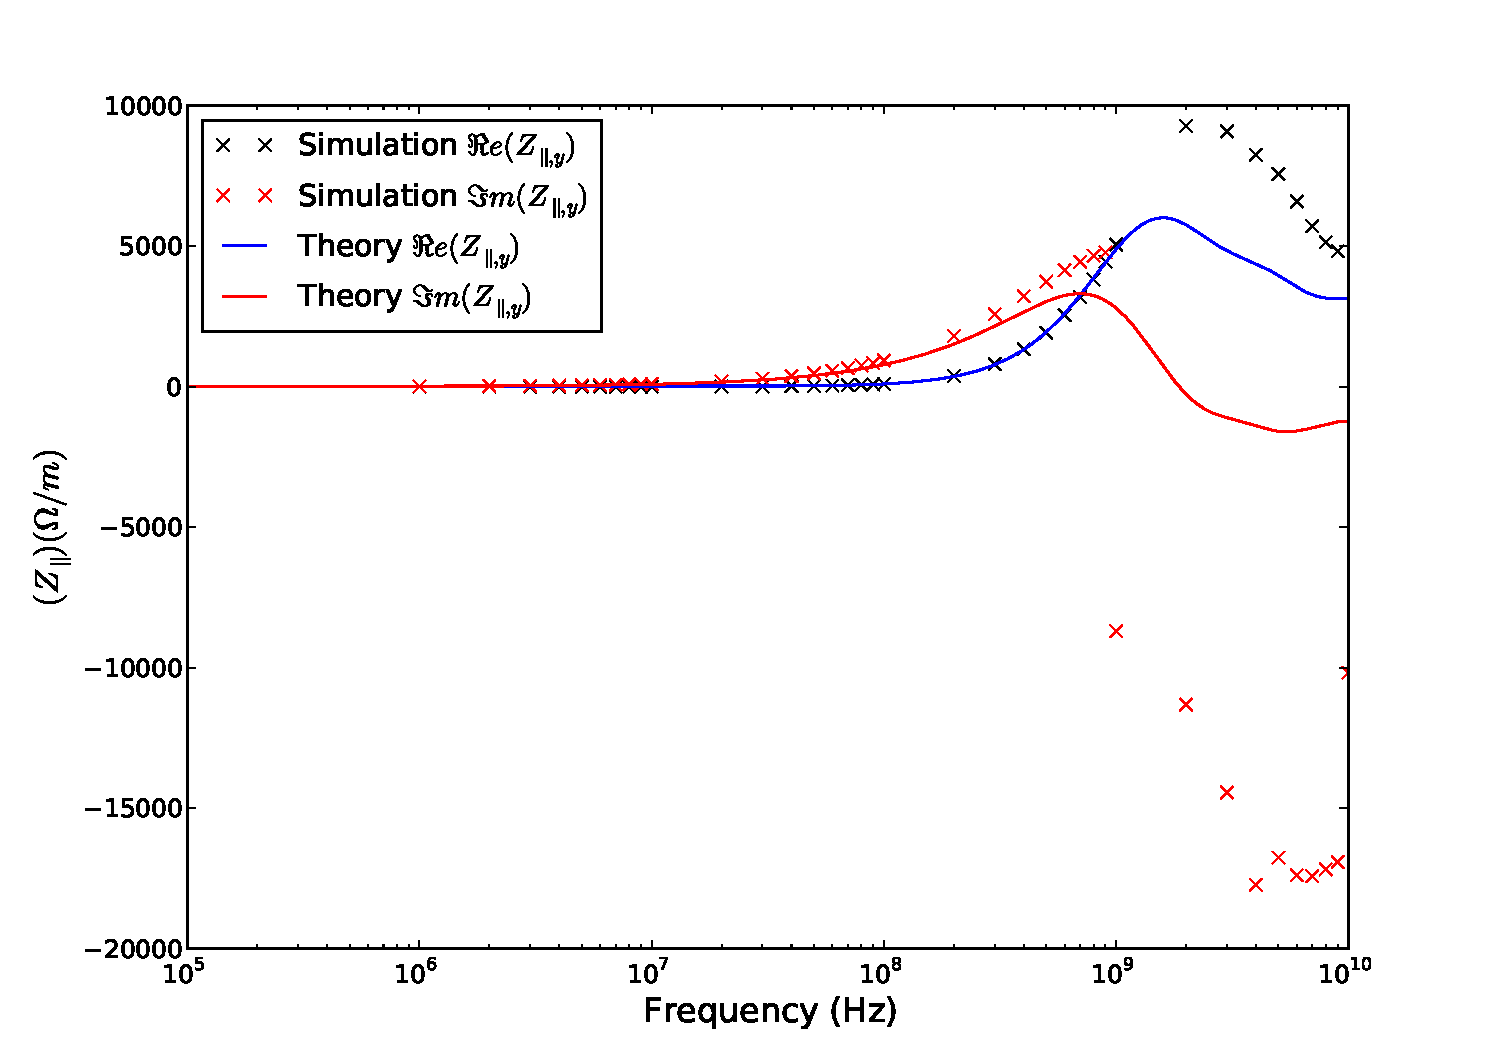
\includegraphics[width=0.5\textwidth]{Bench_Top_Measurements/figures/wire_meas/ferrite_plates/longitudinal-vertical.pdf}
\label{fig:ferrite-plates-long-vert}
}
\caption{The longitudinal impedance of two parallel ferrite plates simulated using a longitudinal coaxial wire. Presented is the impedance as measured in the horizontal plane (\subref{fig:ferrite-plates-long-horz}) and in the vertical plane \subref{fig:ferrite-plates-long-vert}.}
\label{fig:ferrite-plates-long}
\end{figure}

\begin{figure}
\subfigure[]{
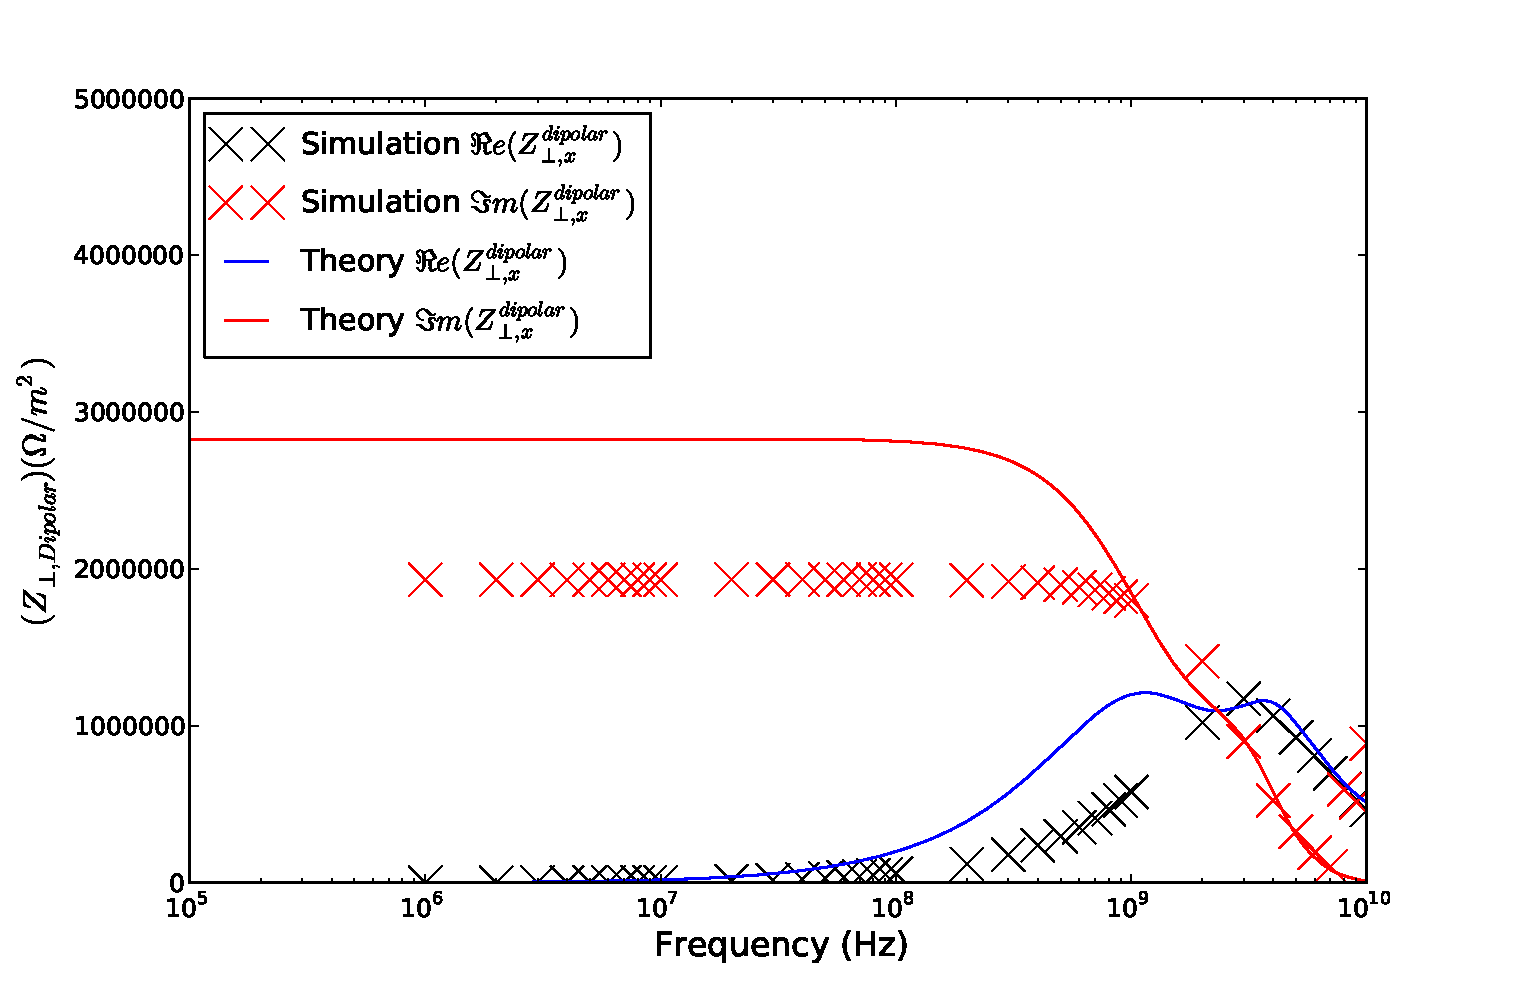
\includegraphics[width=0.5\textwidth]{Bench_Top_Measurements/figures/wire_meas/ferrite_plates/dipolar-horizontal.pdf}
\label{fig:ferrite-plates-dip-horz}
}
\subfigure[]{
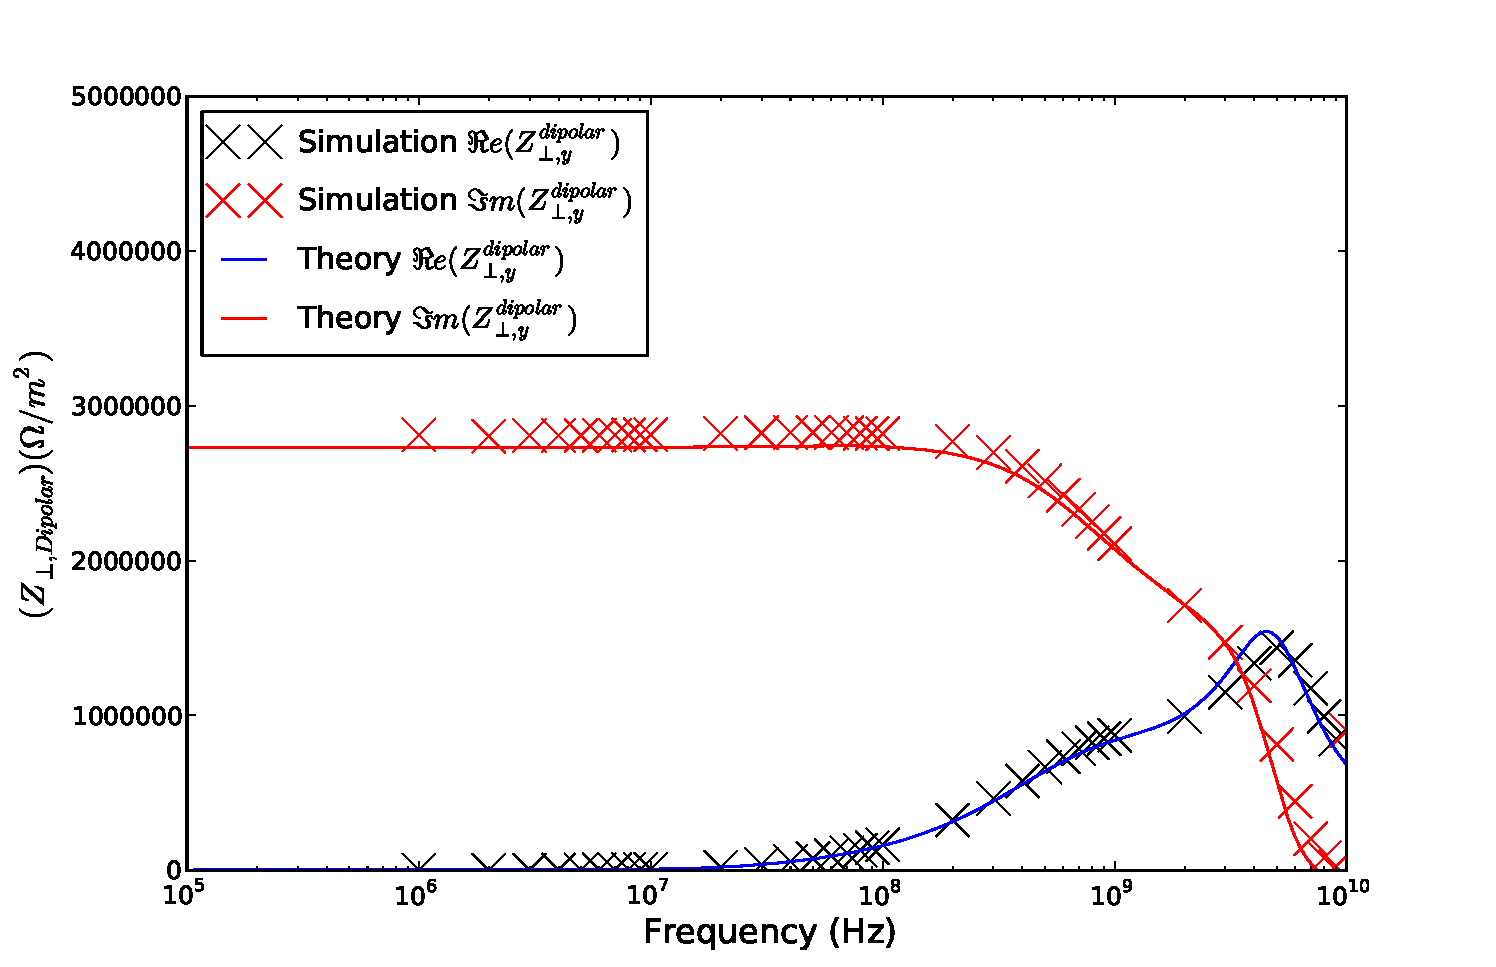
\includegraphics[width=0.5\textwidth]{Bench_Top_Measurements/figures/wire_meas/ferrite_plates/dipolar-vertical.pdf}
\label{fig:ferrite-plates-dip-vert}
}
\caption{The dipolar impedance of two parallel ferrite plates simulated using two longitudinal coaxial wires. Presented are the impedances as measured in the horizontal plane (\subref{fig:ferrite-plates-dip-horz}) and in the vertical plane \subref{fig:ferrite-plates-dip-vert}.}
\label{fig:ferrite-plates-dipolar}
\end{figure}

\begin{figure}
\subfigure[]{
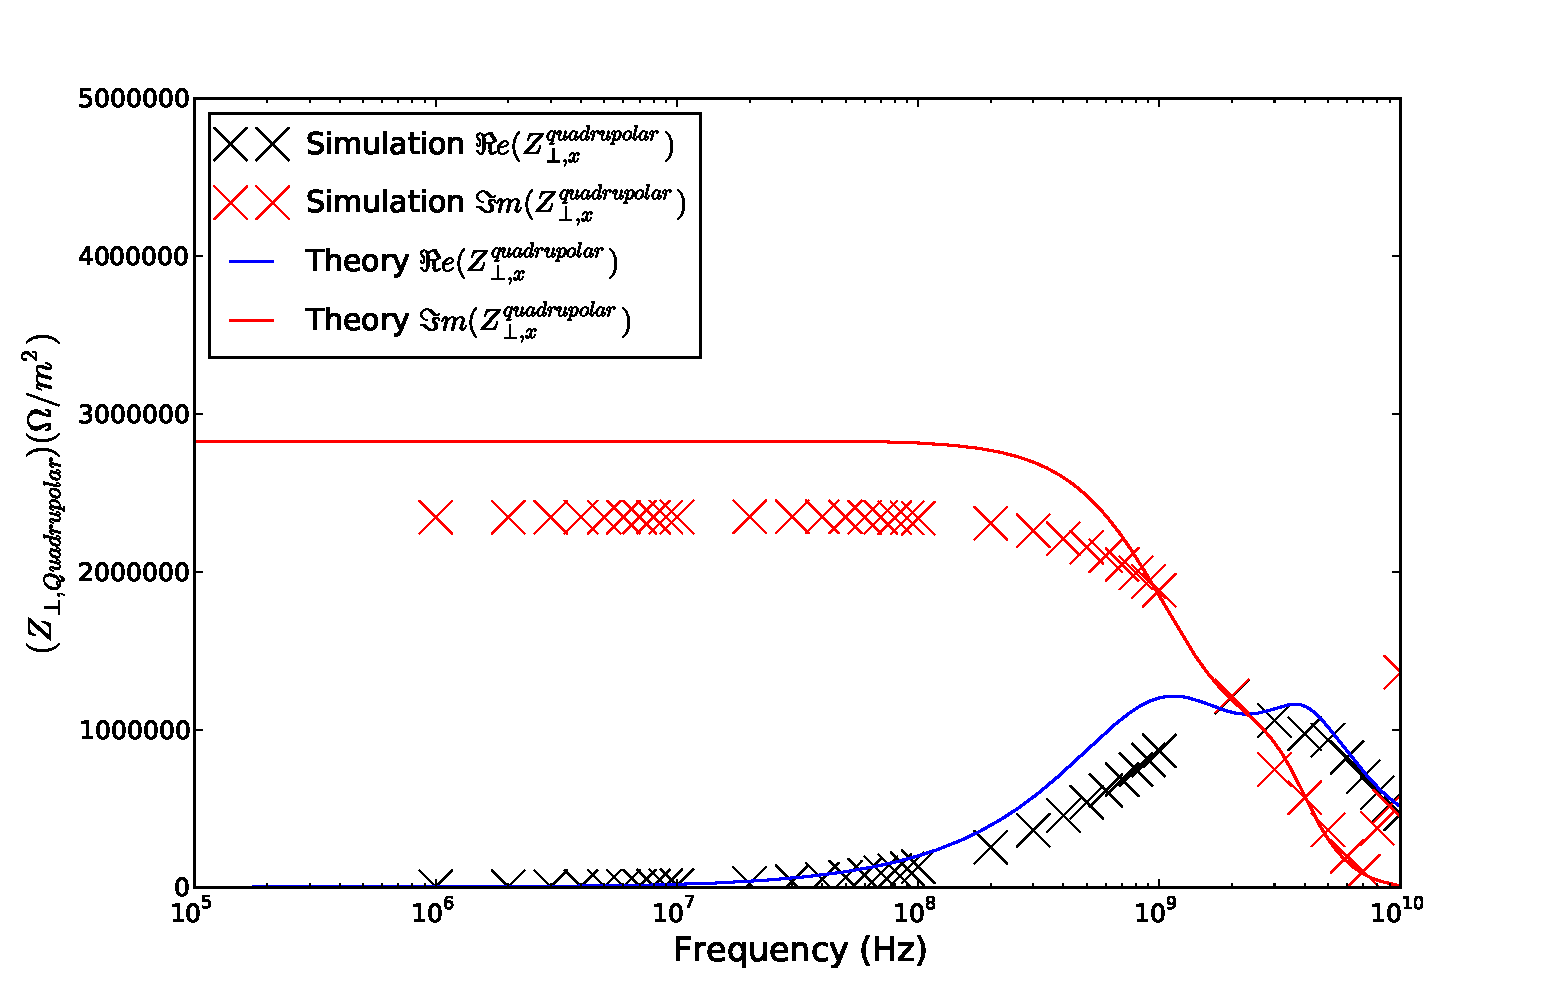
\includegraphics[width=0.5\textwidth]{Bench_Top_Measurements/figures/wire_meas/ferrite_plates/quadrupolar-horizontal.pdf}
\label{fig:ferrite-plates-quad-horz}
}
\subfigure[]{
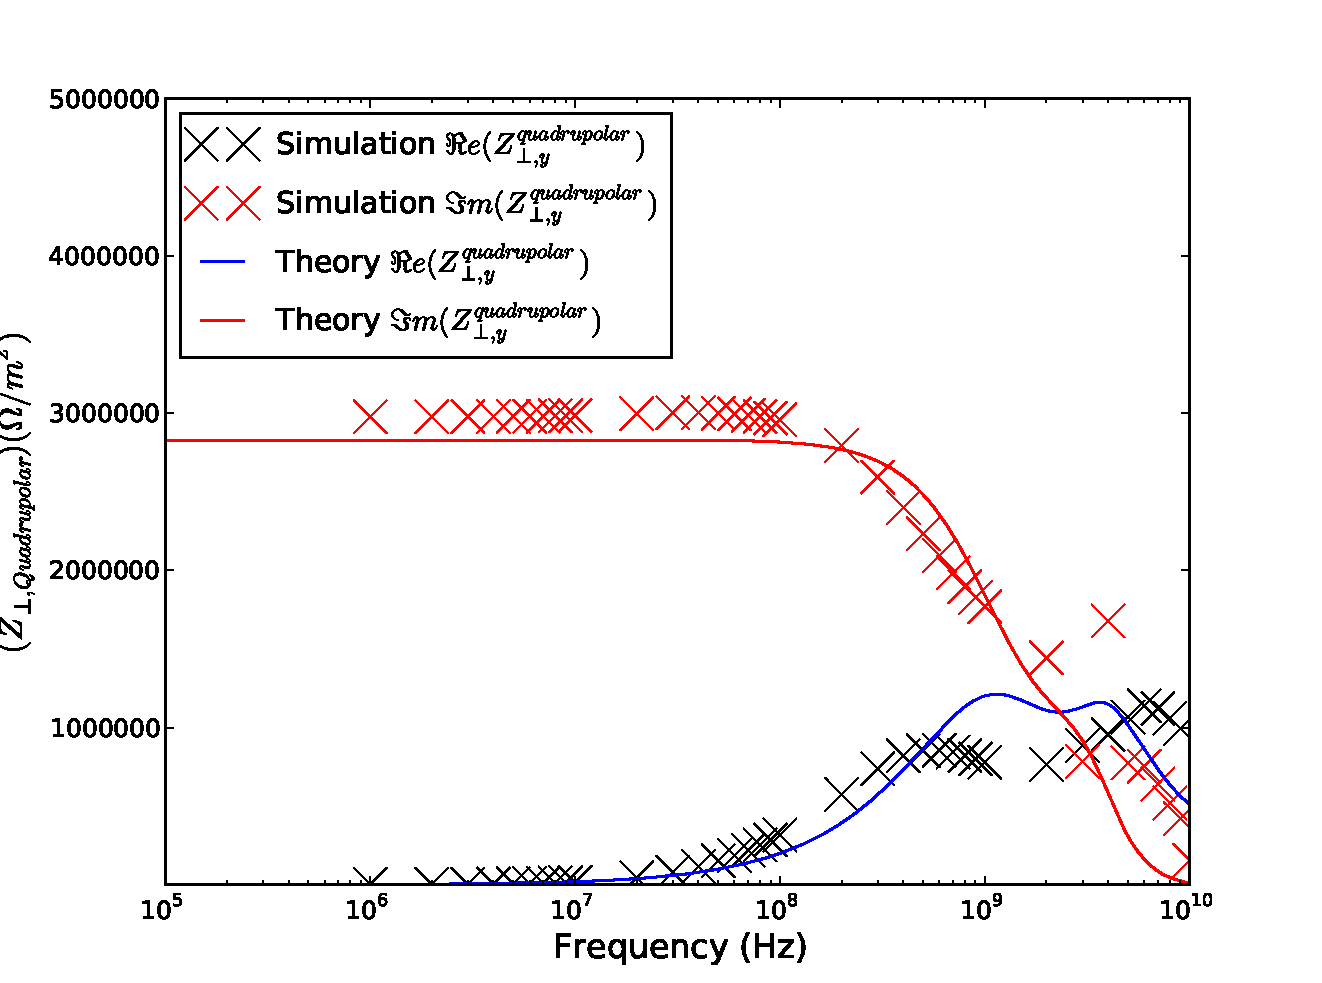
\includegraphics[width=0.5\textwidth]{Bench_Top_Measurements/figures/wire_meas/ferrite_plates/quadrupolar-vertical.pdf}
\label{fig:ferrite-plates-quad-vert}
}
\caption{The quadrupolar impedance of two parallel ferrite plates simulated using a combination of displaced single wire simulated measurements and two wire simulated measurements. Presented is the impedance as measured in the horizontal plane (\subref{fig:ferrite-plates-quad-horz}) and in the vertical plane \subref{fig:ferrite-plates-quad-vert}.}
\label{fig:ferrite-plates-quadrupolar}
\end{figure}

The longitudinal impedance is determined by taking the constant term for a series of simulated displaced wire measurements in both the vertical and horizontal planes is shown in Fig.~\ref{fig:ferrite-plates-long}. It can be seen that in the frequency range below 100MHz the agreement between the coaxial wire results and the analytical results is very good in both the vertical and horizontal plane. Above 100MHz the agreement for the real components is very good for both results, however the imaginary component in the vertical plane displays some substantial disagreement. This is likely due to the high mesh density required to correctly evaluate the phase change along the length of the simulated structure. A higher mesh density may correct this, however limits of computational resource presently make this unfeasible.

The agreement between the simulations of the vertical dipolar impedance and the theoretical model is excellent across all frequencies for both the real and imaginary components. The agreement below 100MHz and above 1GHz is very good for the horizontal dipolar, with some divergence in the constant term of the imaginary impedance. The key difference is the failure of the coaxial method to resolve one of the peaks in the real impedance. The results for the dipolar impedance are shown in Fig.~\ref{fig:ferrite-plates-dipolar}.

The results for the quadrupolar impedance are shown in Fig.~\ref{fig:ferrite-plates-quadrupolar}. The vertical simulations agree well with the theory, correctly identifying the two peaks in the quadrupolar impedance. The agreement for the horizontal simulations with theory is less good. This can be explained by the derivation of the horizontal quadrupolar being highly dependent on the quality of the horizontal dipolar impedance results due to them cancelling each other to form the total transverse impedance. As the horizontal dipolar impedance does not resolve the subpeaks neither does the horizontal quadrupolar impedance calculations.

\subsubsection{Two Parallel Graphite Plates}

For the simulations of measurements of two parallel graphite plates, two different methods were used. Due to the non-ferritic properties of the graphite, it is possible to use Maxwell3D to simulate the power loss at lower frequencies, thus acquiring the real component of the impedance for low frequencies, in addition to using the classical coaxial wire method at higher frequencies in HFSS.

For the simulations of the power loss in Maxwell3D the following parameters were used; for the displaced single wire measurements a wire of 0.5mm radius is modelled, and the following displacement used to acquire the total transverse terms:

\begin{enumerate}
\item{In the horizontal axis -  displaced between -6mm to +6mm at intervals of 2mm}
\item{In the vertical axis - displaced between -4mm to +4mm at intervals of 2mm.}
\end{enumerate}

For the two wire simulations, two wires of radius 0.3mm are modelled, with a seperation of 8mm in the x-dimension, and 4mm in the y-dimension. Five simulation configurations are used as described below:

\begin{enumerate}
\item{an adaptive mesh generation set to a convergence criterion of $S_{21}$ diverging by less than 0.005 between two subsequent solutions, at an adaptive frequency of 20kHz solving to a second order basis. A discrete frequency sweep is then carried out in the range 1-10kHz at 1kHz intervals.}
\item{an adaptive mesh generation set to a convergence criterion of $S_{21}$ diverging by less than 0.005 between two subsequent solutions, at an adaptive frequency of 200kHz solving to a second order basis. A discrete frequency sweep is then carried out in the range 10-100kHz at 10kHz intervals.}
\item{an adaptive mesh generation set to a convergence criterion of $S_{21}$ diverging by less than 0.005 between two subsequent solutions, at an adaptive frequency of 2MHz solving to a second order basis. A discrete frequency sweep is then carried out in the range 100kHz-1MHz at 100kHz intervals.}
\item{an adaptive mesh generation set to a convergence criterion of $S_{21}$ diverging by less than 0.005 between two subsequent solutions, at an adaptive frequency of 10MHz solving to a second order basis. A discrete frequency sweep is then carried out in the range 1-10MHz at 1MHz intervals.}
\item{an adaptive mesh generation set to a convergence criterion of $S_{21}$ diverging by less than 0.005 between two subsequent solutions, at an adaptive frequency of 100MHz solving to a second order basis. A discrete frequency sweep is then carried out in the range 10-100MHz at 10MHz intervals.}
\end{enumerate}

These parameters are used to benefit from an appropriate mesh count for the given frequency range, thus increasing simulation speed by not using a high density mesh at frequencies where no benefits would be gained.

For the simulations of the single displaced wire in HFSS the following parameters were used; for the displaced single wire measurements a wire of 0.3mm in radius is modelled, and the following displacements to acquire the total transverse terms:

\begin{enumerate}
\item{In the horizontal axis -  displaced between -6mm to +6mm at intervals of 2mm}
\item{In the vertical axis - displaced between -4mm to +4mm at intervals of 2mm.}
\end{enumerate}

For the two wire simulations, two wires of radius 0.3mm are modelled, with a seperation of 4mm in the x-dimension, and 3mm in the y-dimension. Three simulations configuration are used as described below:

\begin{enumerate}
\item{an adaptive mesh generation set to a convergence criterion of $S_{21}$ diverging by less than 0.005 between two subsequent solutions, at an adaptive frequency of 20MHz solving to a second order basis. A discrete frequency sweep is then carried out in the range 1-10MHz at 1MHz intervals.}
\item{an adaptive mesh generation set to a convergence criterion of $S_{21}$ diverging by less than 0.005 between two subsequent solutions, at an adaptive frequency of 200MHz solving to a second order basis. A discrete frequency sweep is then carried out in the range 10-100MHz at 10MHz intervals.}
\item{an adaptive mesh generation set to a convergence criterion of $S_{21}$ diverging by less than 0.005 between two subsequent solutions, at an adaptive frequency of 2GHz solving to a second order basis. A discrete frequency sweep is then carried out in the range 100MHz-1GHz at 100MHz intervals.}
\end{enumerate}

As before these parameters are used to benefit from an appropriate mesh count for the given frequency range, thus increasing simulation speed by not using a high density mesh at frequencies where no benefits would be gained.

\begin{figure}
\subfigure[]{
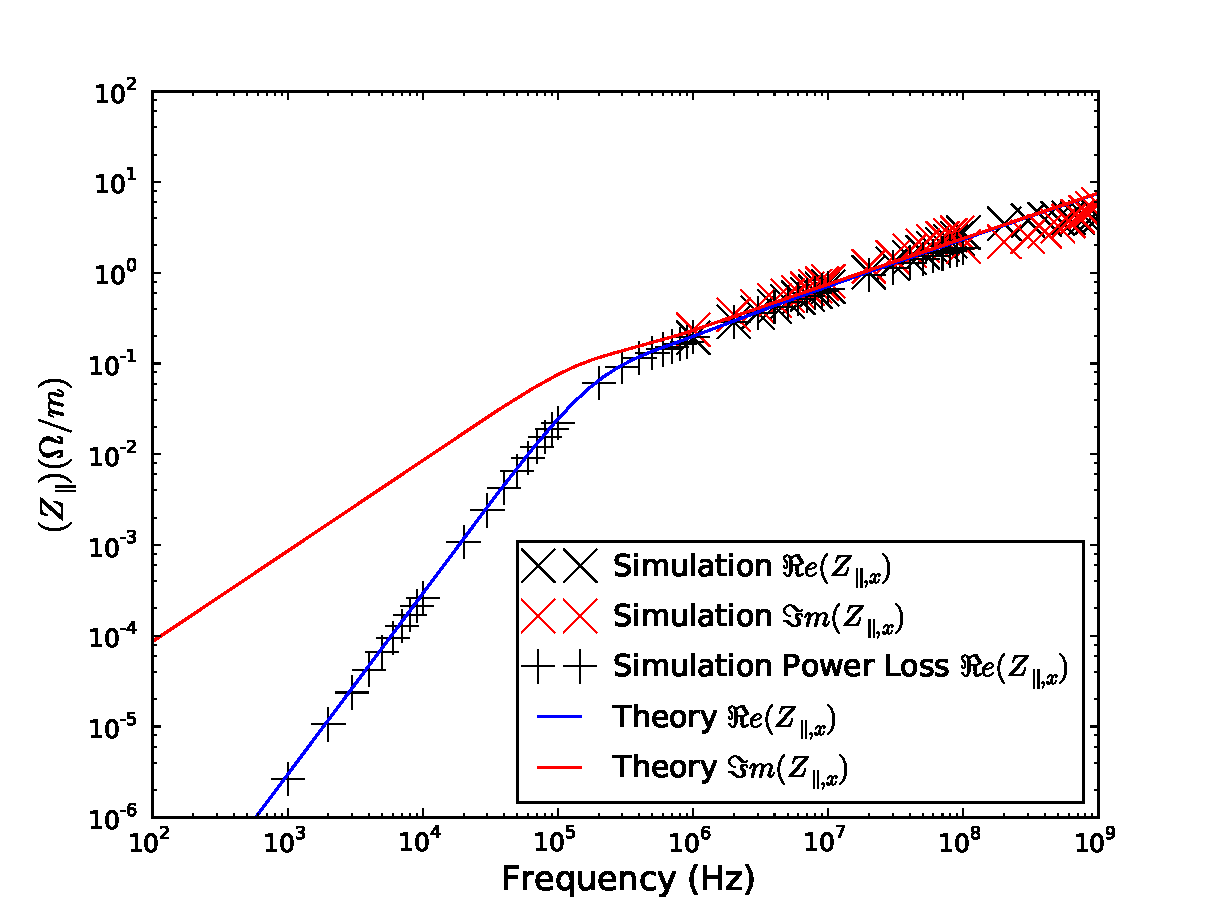
\includegraphics[width=0.5\textwidth]{Bench_Top_Measurements/figures/wire_meas/graphite_plates/longitudinal-horizontal.pdf}
\label{fig:graph-plates-long-horz}
}
\subfigure[]{
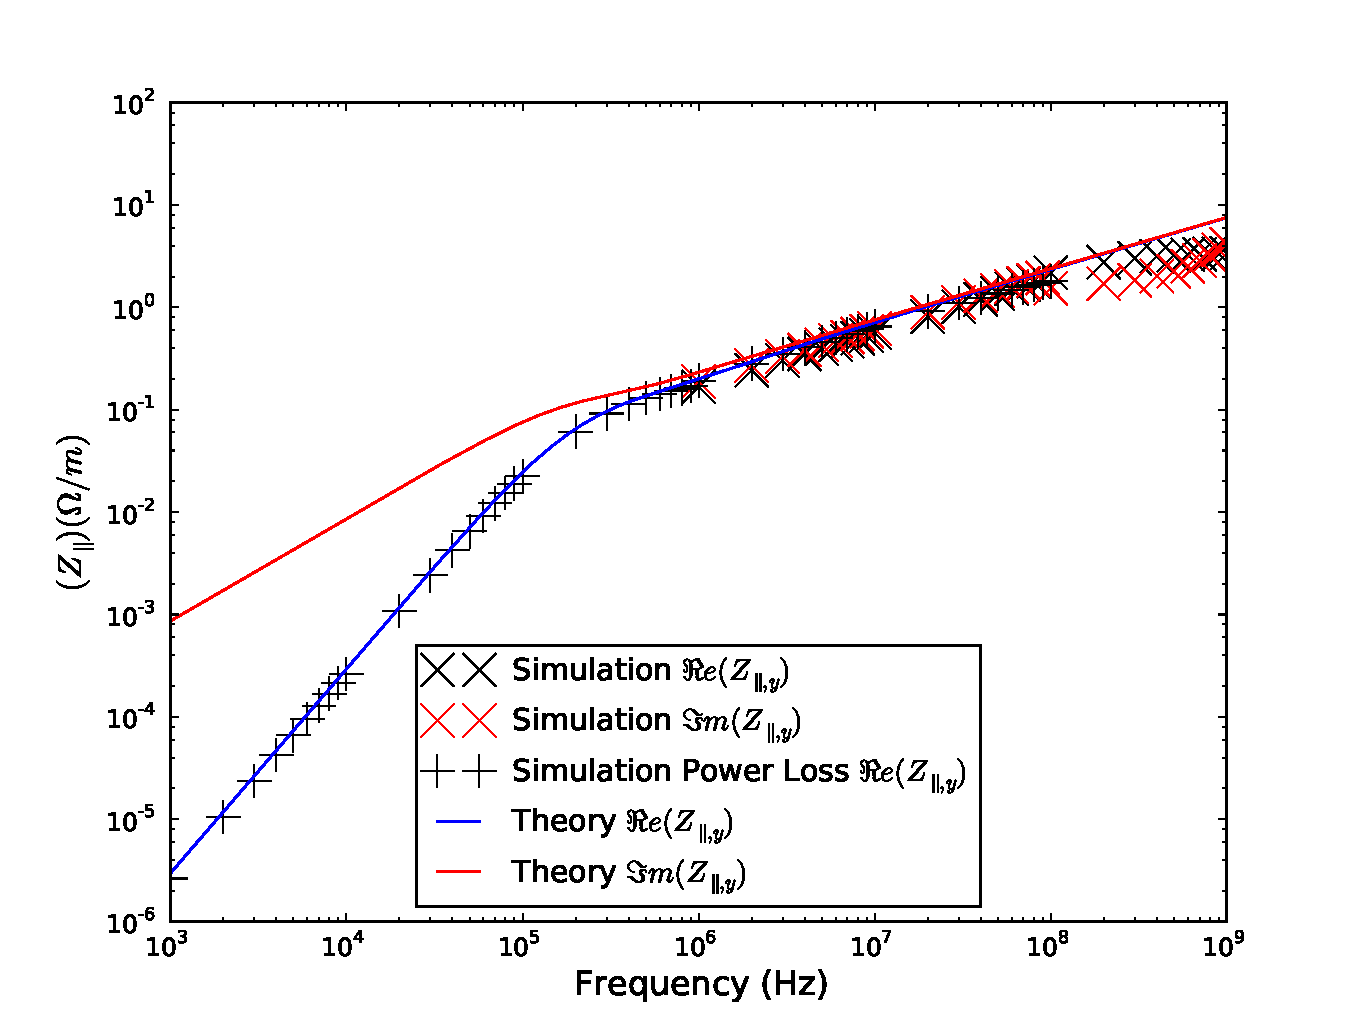
\includegraphics[width=0.5\textwidth]{Bench_Top_Measurements/figures/wire_meas/graphite_plates/longitudinal-vertical.pdf}
\label{fig:graph-plates-long-vert}
}
\caption{The longitudinal impedance of two parallel graphite plates as measured by taking the constant term of a quadratic equation fitted to a series of displaced single wire simulated measurements. Shown are simulated measurements acquired from fitting displacements in \subref{fig:graph-plates-long-horz} horizontal axis and in \subref{fig:graph-plates-long-vert} the vertical axis.}
\label{fig:graph-plates-long-imp}
\end{figure}

\begin{figure}
\subfigure[]{
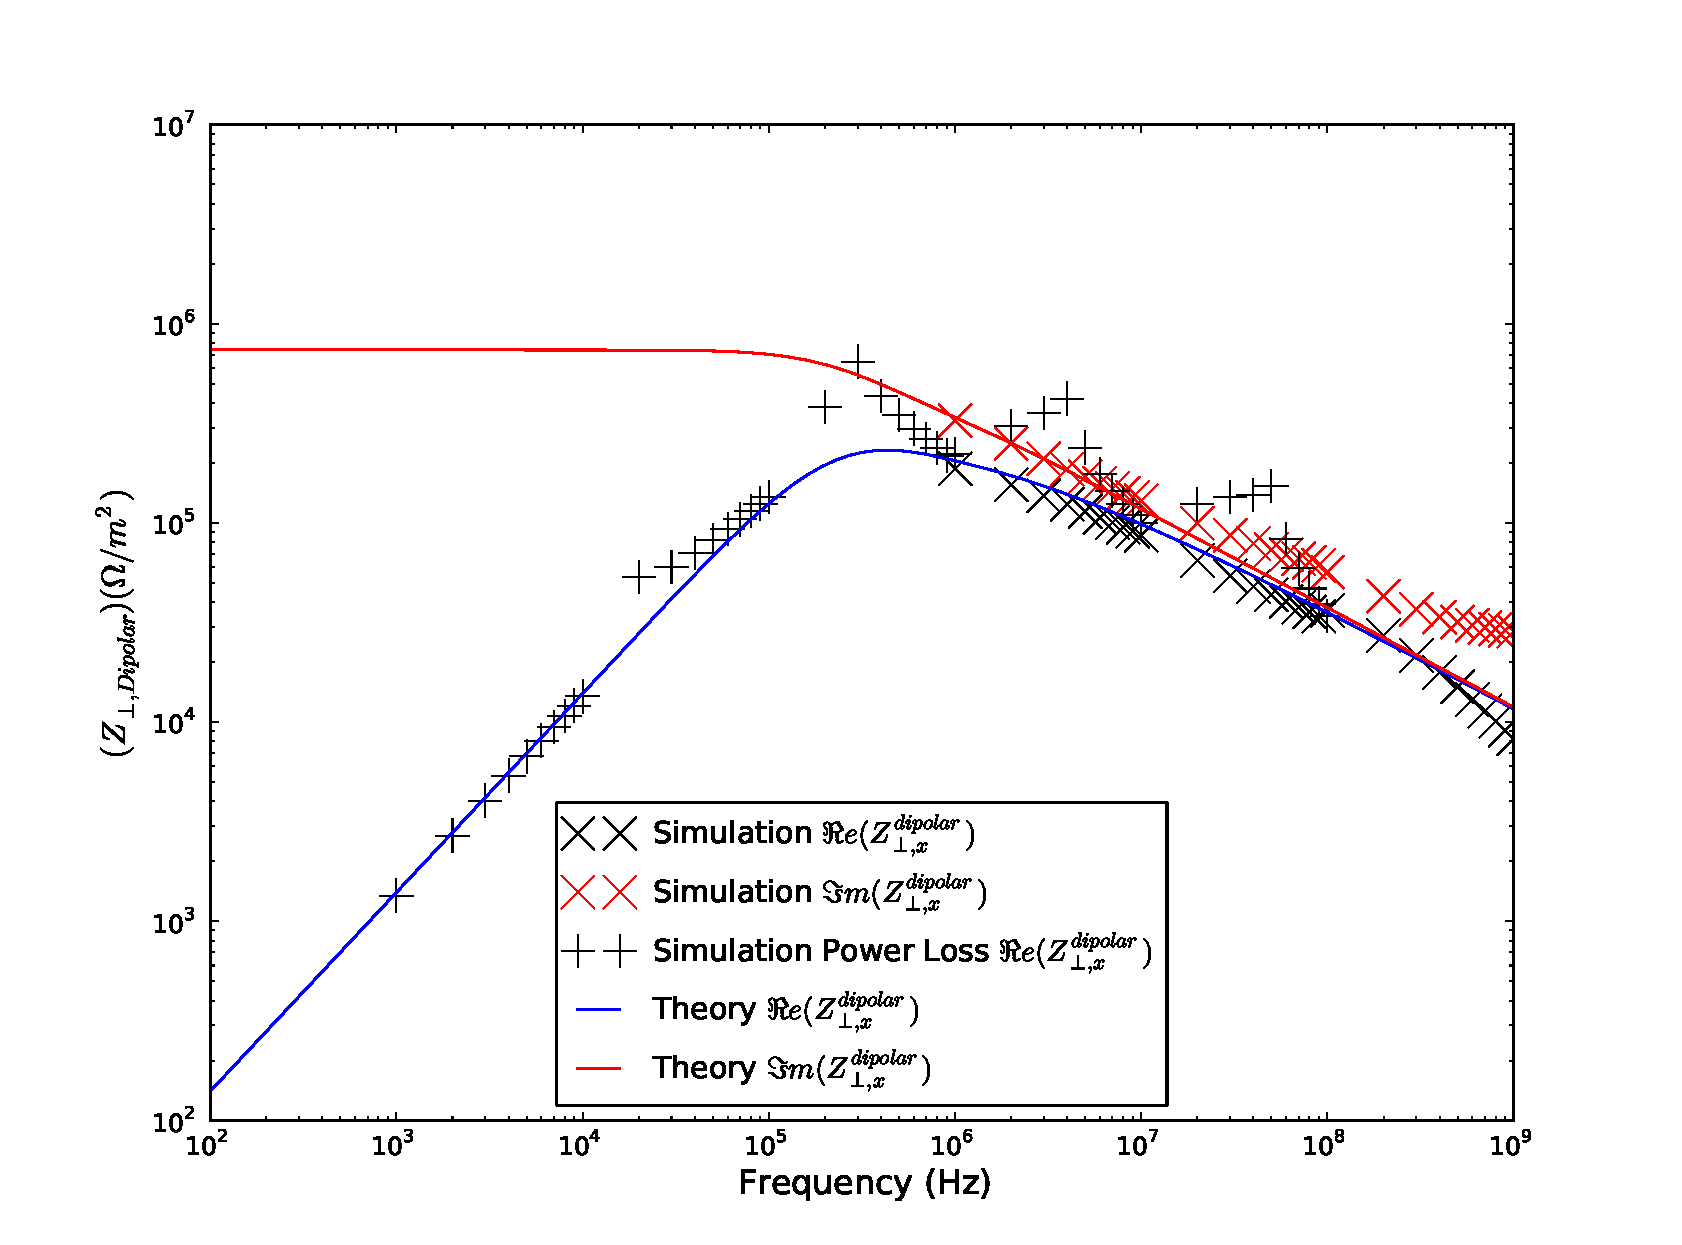
\includegraphics[width=0.5\textwidth]{Bench_Top_Measurements/figures/wire_meas/graphite_plates/dipolar-horizontal.pdf}
\label{fig:graph-plates-dip-horz}
}
\subfigure[]{
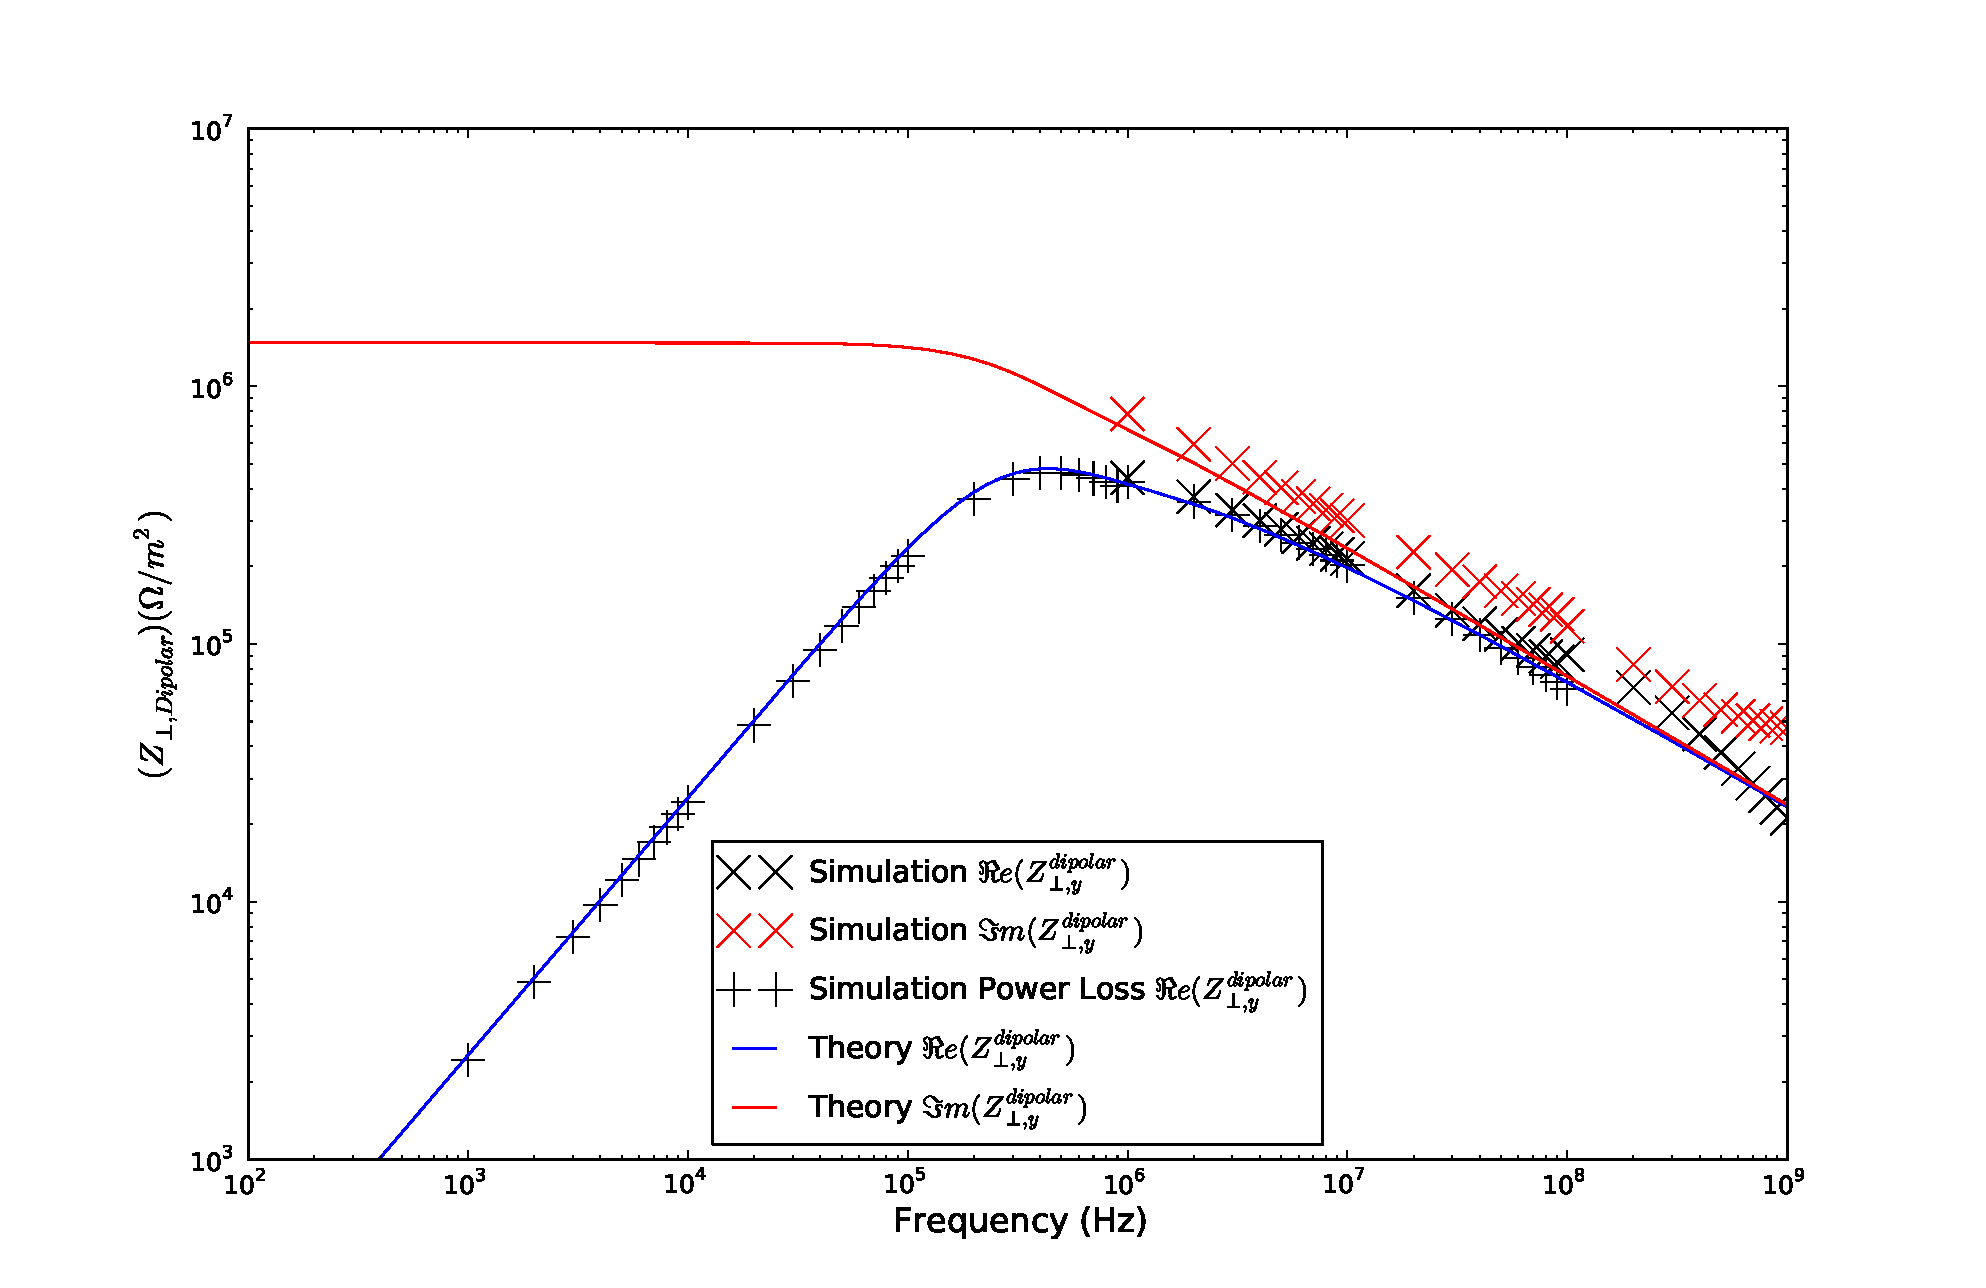
\includegraphics[width=0.5\textwidth]{Bench_Top_Measurements/figures/wire_meas/graphite_plates/dipolar-vertical.pdf}
\label{fig:graph-plates-dip-vert}
}
\caption{The dipolar impedance of two parallel graphite plates measured using two longitudinal coaxial wires. Presented is the impedance as measured in the horizontal plane (\subref{fig:graph-plates-dip-horz}) and in the vertical plane \subref{fig:graph-plates-dip-vert}.}
\label{fig:graph-plates-dipolar}
\end{figure}

\begin{figure}
\begin{center}
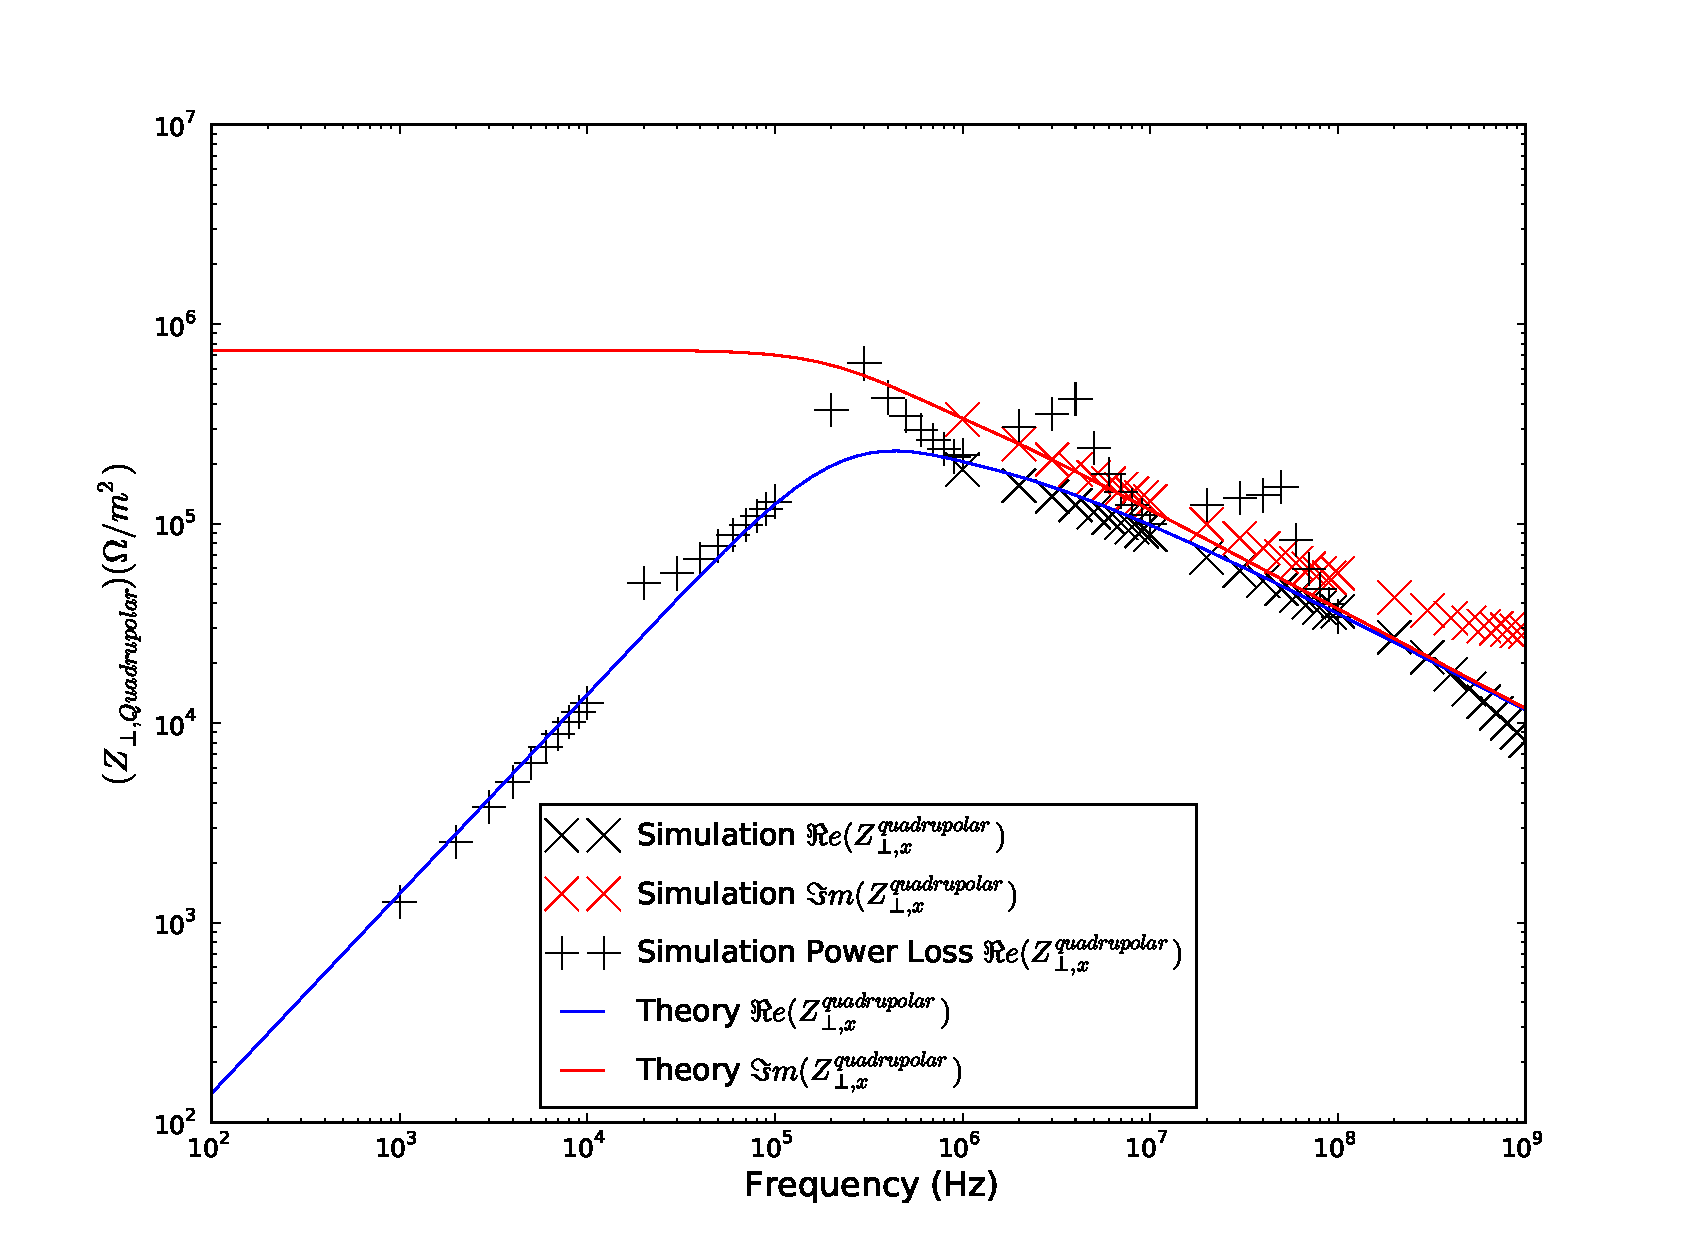
\includegraphics[width=0.75\textwidth]{Bench_Top_Measurements/figures/wire_meas/graphite_plates/quadrupolar-horizontal.pdf}
\end{center}
\caption{The quadrupolar impedance of two parallel graphite plates measured using a combination of displaced single wire measurements and two wire mesurements.}
\label{fig:graph-plates-quadrupolar}
\end{figure}

The longitudinal impedance in Fig.~\ref{fig:graph-plates-long-imp}. It can be seen that the agreement for both the real component is excellent across the entire frequency range, for simulations using both the classical coaxial wire method and the power loss method of Maxwell3D. The agreement is also good for the imaginary component over much of the frequency range, becoming worse above 100MHz. This is likely due to insufficient mesh density to catch the relatively small phase shift at this frequency range.

The agreement between simulations and theory for the vertical dipolar impedance can be seen to be very good over the entire frequency range also (see Fig.~\ref{fig:graph-plates-dip-vert}). The results at low frequencies (below 100kHz) for the power loss method and at all frequencies for the classical coaxial wire method for the horizontal dipolar impedance agree very well with theory (see Fig.~\ref{fig:graph-plates-dip-horz}). The quadrupolar impedance is shown in Fig.~\ref{fig:graph-plates-quadrupolar}, and again the agreement between the simulated measurements and theory can be seen to be good over the entire frequency range, using both the power loss method and the classical coaxial wire method. However, the power loss method does predict peaks at the lower part of each frequency sweep that are not predicted in either tha theoretical model or the measurements with the coaxial wire method in HFSS.

\subsubsection{C-Core Ferrite Kicker}

To test the measurement method for an asymmetric structure a model of the C-core ferrite kicker magnet was used, as shown in Fig.\ref{fig:zannini-model}, the analytical details of which are given in \cite{Zannini:cCoreFerrite}. Key in this type of structure is that it predicts a non-zero constant transverse impedance term as well as the quadrupolar terms, thus we may completely evaluate the asymmetric measurement method. For these simulations a structure of $a=15$mm, $r=20$mm, $\theta = \pi / 2$, and $100$mm in length was used. Simulations were carried out using the classical coaxial wire method as simulated in HFSS.

The following parameters were used for the simulations; wire of 0.2mm in radius, and the following displacement used to acquire the total transverse terms:

\begin{enumerate}
\item{In the horizontal axis -  displaced between -5mm to +5mm at intervals of 1mm.}
\item{In the vertical axis - displaced between -5mm to +5mm at intervals of 1mm.}
\end{enumerate}

For the two wire simulations, two wires of radius 0.2mm are modelled, with a separation of 2mm in the x-dimension, and 2mm in the y-dimension. Four simulation configurations were used which are described below:

\begin{enumerate}
\item{an adaptive mesh generation set to a convergence criterion of $S_{21}$ diverging by less than 0.005 between two subsequent solutions, at an adaptive frequency of 20MHz solving to a second order basis. A discrete frequency sweep is then carried out in the range 1-10MHz at 1MHz intervals.}
\item{an adaptive mesh generation set to a convergence criterion of $S_{21}$ diverging by less than 0.005 between two subsequent solutions, at an adaptive frequency of 200MHz solving to a second order basis. A discrete frequency sweep is then carried out in the range 10-100MHz at 10MHz intervals.}
\item{an adaptive mesh generation set to a convergence criterion of $S_{21}$ diverging by less than 0.005 between two subsequent solutions, at an adaptive frequency of 2GHz solving to a second order basis. A discrete frequency sweep is then carried out in the range 100MHz-1GHz at 100MHz intervals.}
\item{an adaptive mesh generation set to a convergence criterion of $S_{21}$ diverging by less than 0.005 between two subsequent solutions, at an adaptive frequency of 10GHz solving to a second order basis. A discrete frequency sweep is then carried out in the range 1-10GHz at 1GHz intervals.}
\end{enumerate}

These parameters are used to benefit from an appropriate mesh count for the given frequency range, thus increasing simulation speed by not using a high density mesh at frequencies where no benefits would be gained.

\begin{figure}
\subfigure[]{
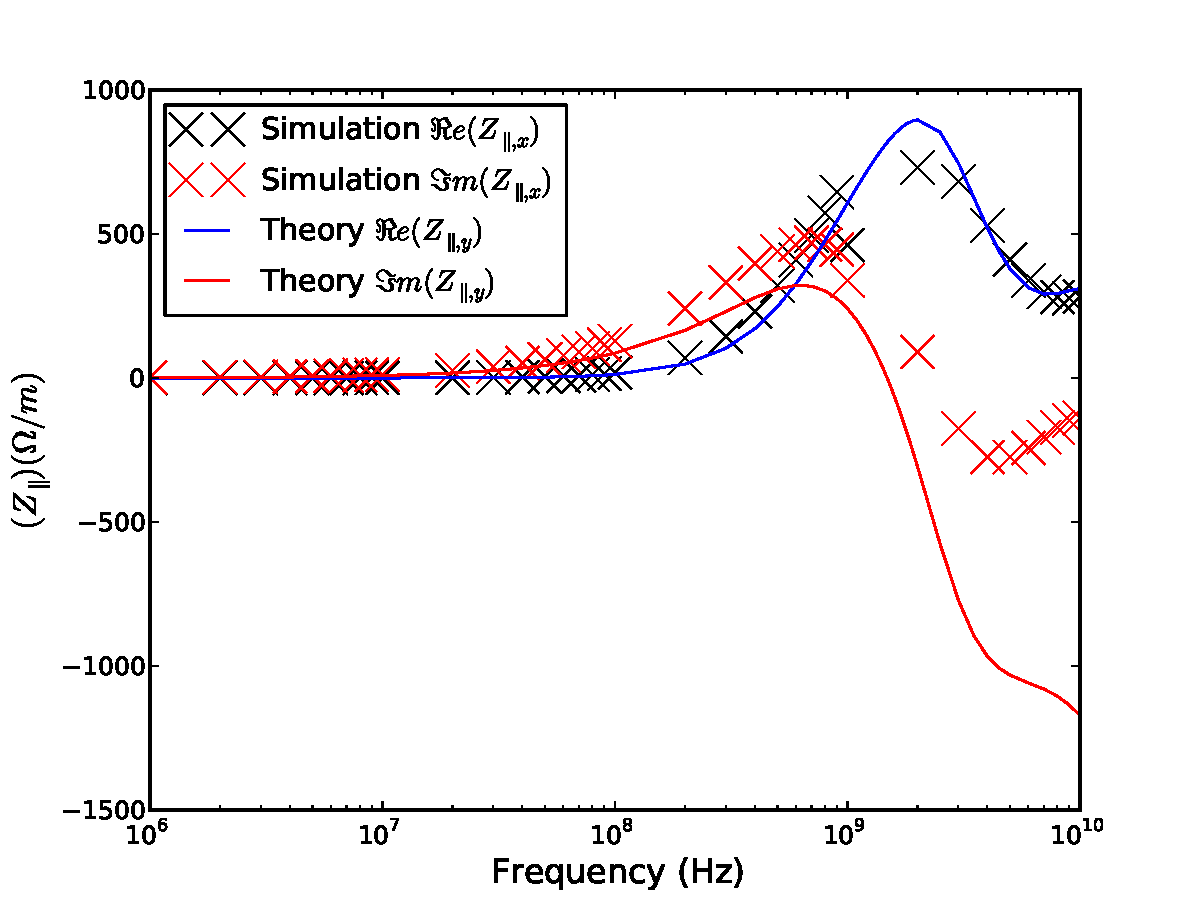
\includegraphics[height=0.35\textwidth]{Bench_Top_Measurements/figures/wire_meas/ferrite-c-core/longitudinal-impedance.pdf}
\label{fig:c-core-longitudinal}
}
\subfigure[]{
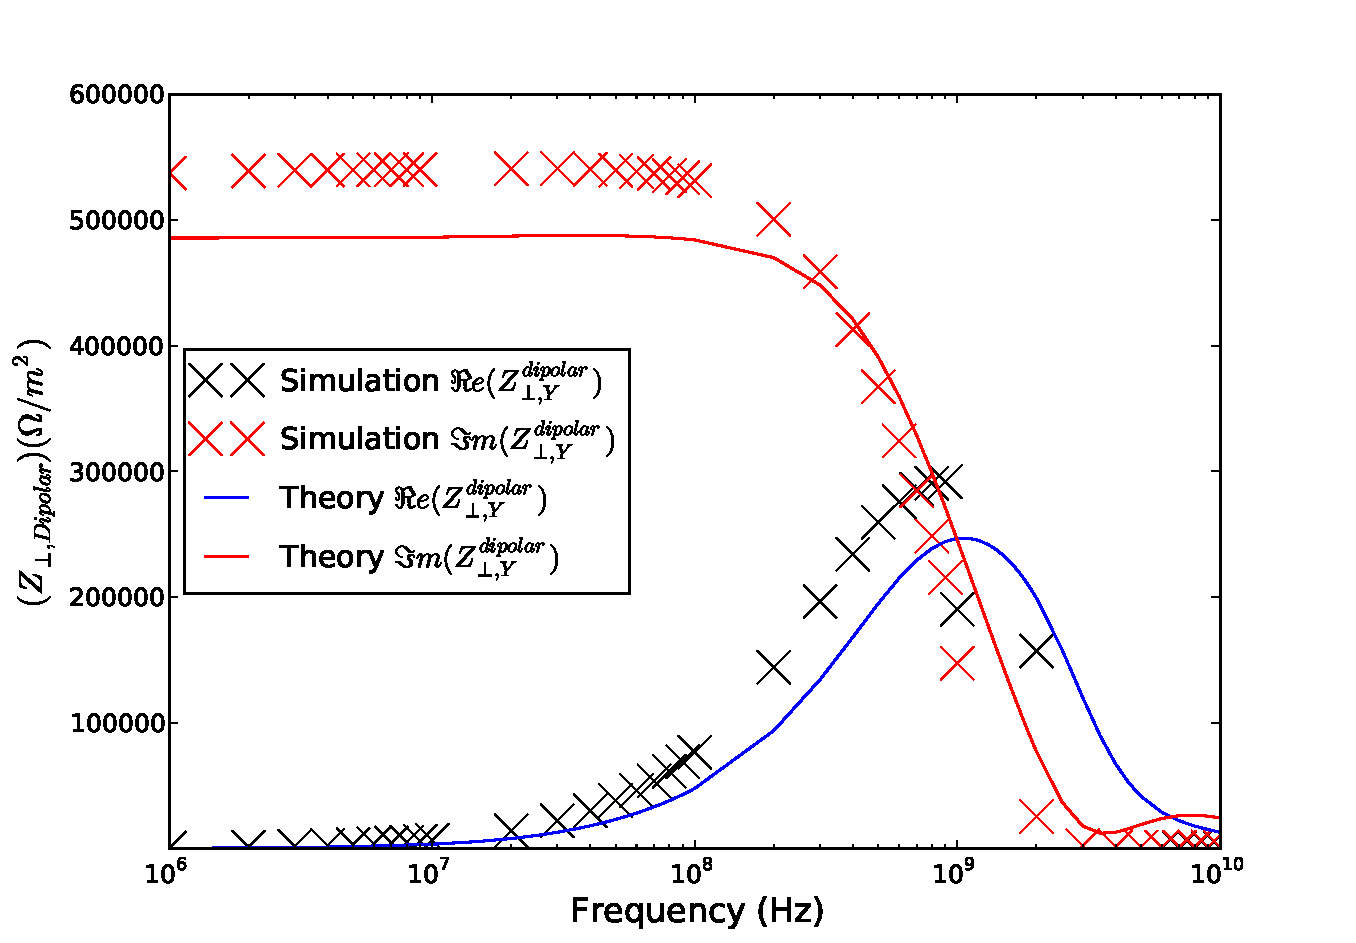
\includegraphics[height=0.35\textwidth]{Bench_Top_Measurements/figures/wire_meas/ferrite-c-core/dipolar-vertical-impedance.pdf}
\label{fig:c-core-dipolar}
}
\subfigure[]{
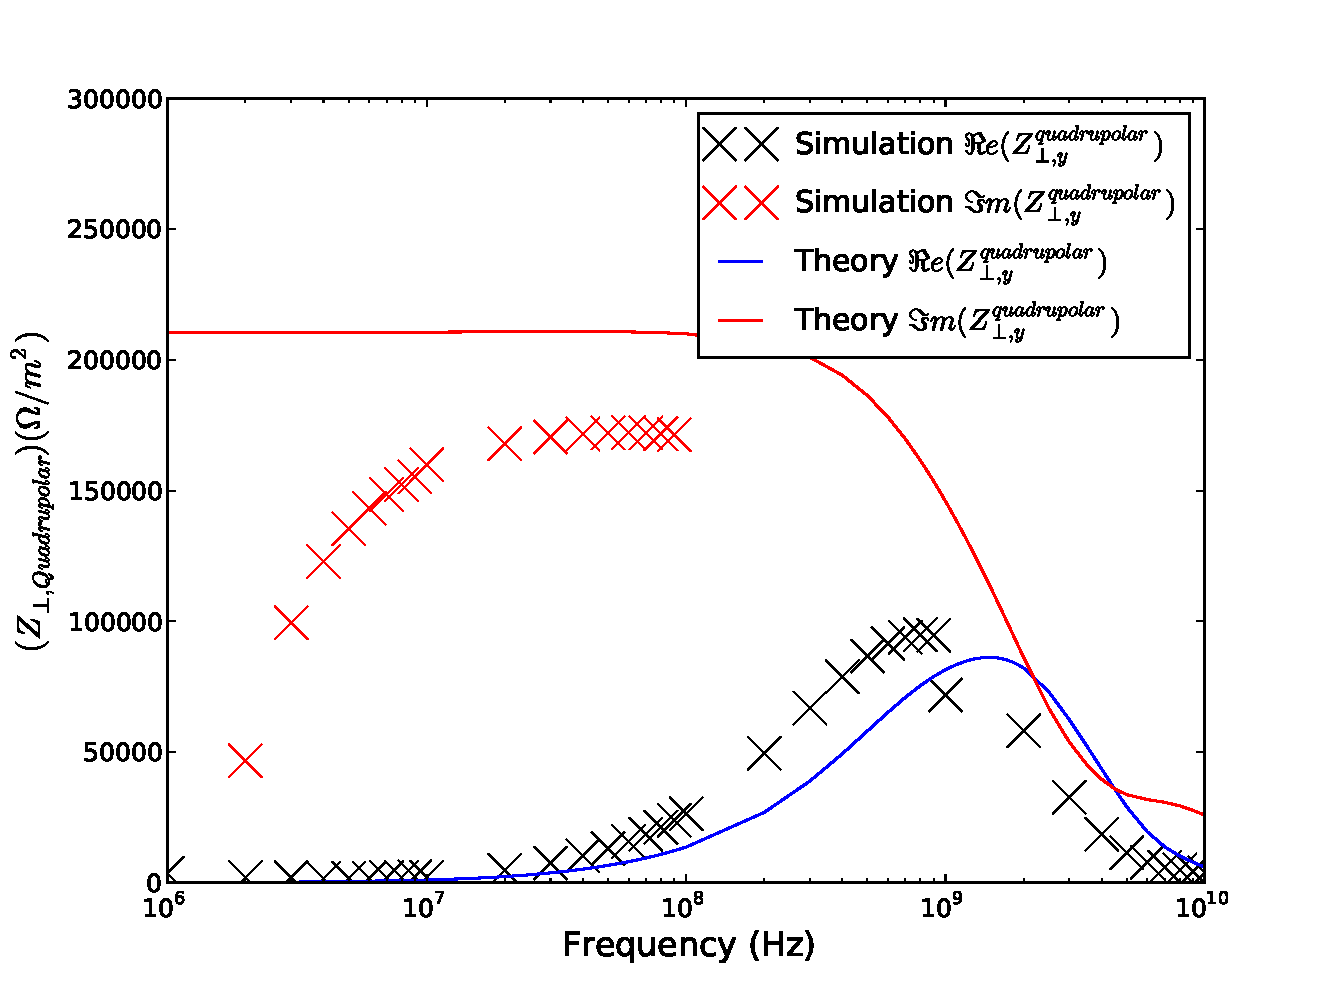
\includegraphics[height=0.35\textwidth]{Bench_Top_Measurements/figures/wire_meas/ferrite-c-core/quadrupolar-vertical-impedance.pdf}
\label{fig:c-core-quadrupolar}
}
\subfigure[]{
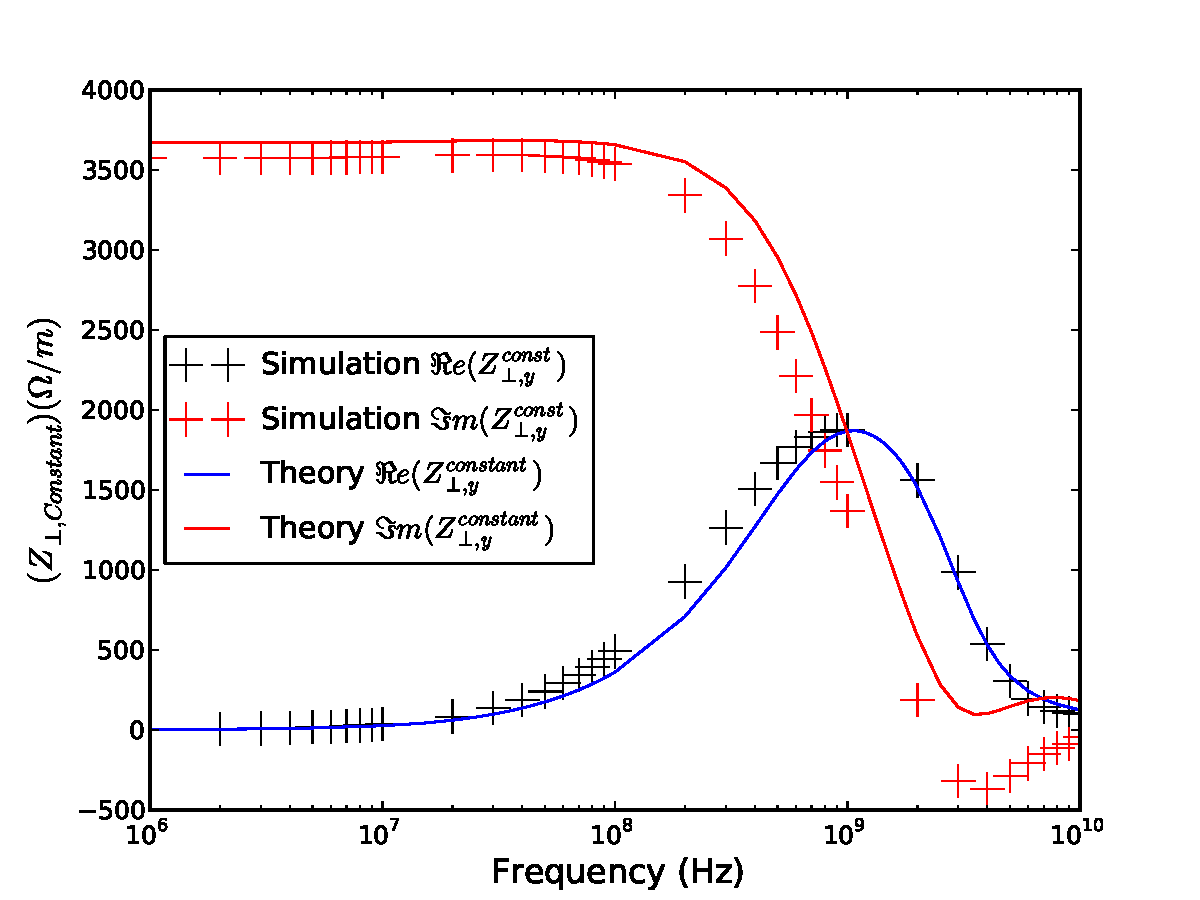
\includegraphics[height=0.35\textwidth]{Bench_Top_Measurements/figures/wire_meas/ferrite-c-core/constant-vertical-impedance.pdf}
\label{fig:c-core-constant}
}
\caption{The impedance of the C-core ferrite kicker as acquired by simulating the classical coaxial wire method in HFSS. Shown is the \subref{fig:c-core-longitudinal} longitudinal impedance, \subref{fig:c-core-dipolar} the dipolar impedance, \subref{fig:c-core-quadrupolar} the quadrupolar impedance and \subref{fig:c-core-constant} the constant transverse impedance.}
\end{figure}

It can be seen that the longitudinal impedance agrees well over the entire frequency range below 1GHz (Fig.~\ref{fig:c-core-longitudinal}). The analytical calculations breakdown above 1GHz due to the family of Bessel functions used for the calculations being optimised for low frequency calculations. Similarly the agreement for the dipolar impedance can be seen to be exceptionally good over the majority of the frequency range, with an increasing descrepency at high frequencies (Fig.~\ref{fig:c-core-dipolar}).

To test the asymmetric method we should look at the constant and quadrupolar terms. In this case it can be seen that the agreement with the constant transverse term is exceptionally good across the entire frequency range (Fig.~\ref{fig:c-core-constant}). The agreement for the quadrupolar impedance is good in the range of frequencies below 1GHz. Above this the unsuitability of the family of Bessel functions used for this frequency range becomes more apparents and the simulated and analytical results diverge.

It can be seen that the proposed asymmetric method can replicate the beam coupling impedance of an asymmetric structure, correctly predicting both longitudinal and transverse (dipolar, quadrupolar and constant) terms below 1GHz. 

\section{High Q-factor Impedances}

For high Q-factor impedances, such as cavity impedances, it is not appropriate to use a coaxial wire method to measure the impedance due to the large perturbation of the boundary conditions that it causes \cite{Masullo:StretchedWire}, in particular below the cut-off frequency of the connecting beam pipes. This is due to the presence of the coaxial wire reducing the cut-off frequency to 0Hz, thus allowing propogation losses at all frequencies rather than just above cut-off. To illustrate this, we can consider the total Q of a cavity to be related to the "trapped" cavity mode Q and the propogation losses as;

\begin{equation}
\frac{1}{Q_{total}} = \frac{1}{Q_{cavity}} + \frac{1}{Q_{prop}}
\end{equation}

During excitation by a charged particle beam, propogation losses do not exist below the cutoff frequency and thus $Q_{prop} = 0$. However, the addition of the coaxial wire causes these propogation losses to occur at all frequencies. Importantly, the Q-factor of these propogation losses is of a similar magnitude or smaller than that of the cavity resonance, leading to a great distortion of the measured Q. Similarly, the perturbation of the conductive wire in the centre of the structure leads to a shift in the resonance frequency of the cavity modes.  This has been well studied in \cite{Masullo:StretchedWire}, an example of which is given in Fig.~\ref{fig:cav-wire-tans}.


\begin{figure}
\subfigure[]{
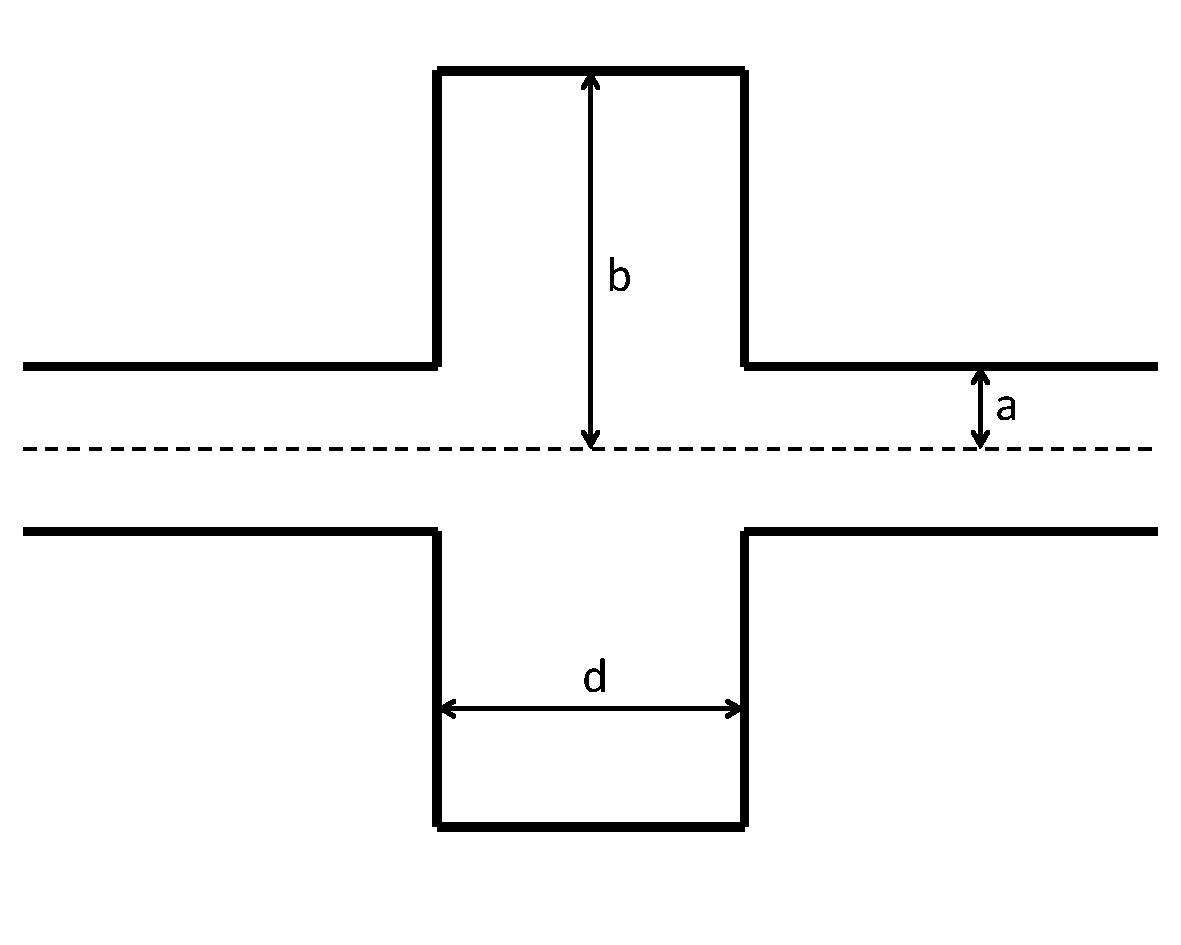
\includegraphics[width=0.5\linewidth]{figures/cavity_beampipe.pdf}
\label{fig:cavity_beampipe}
}
\subfigure[]{
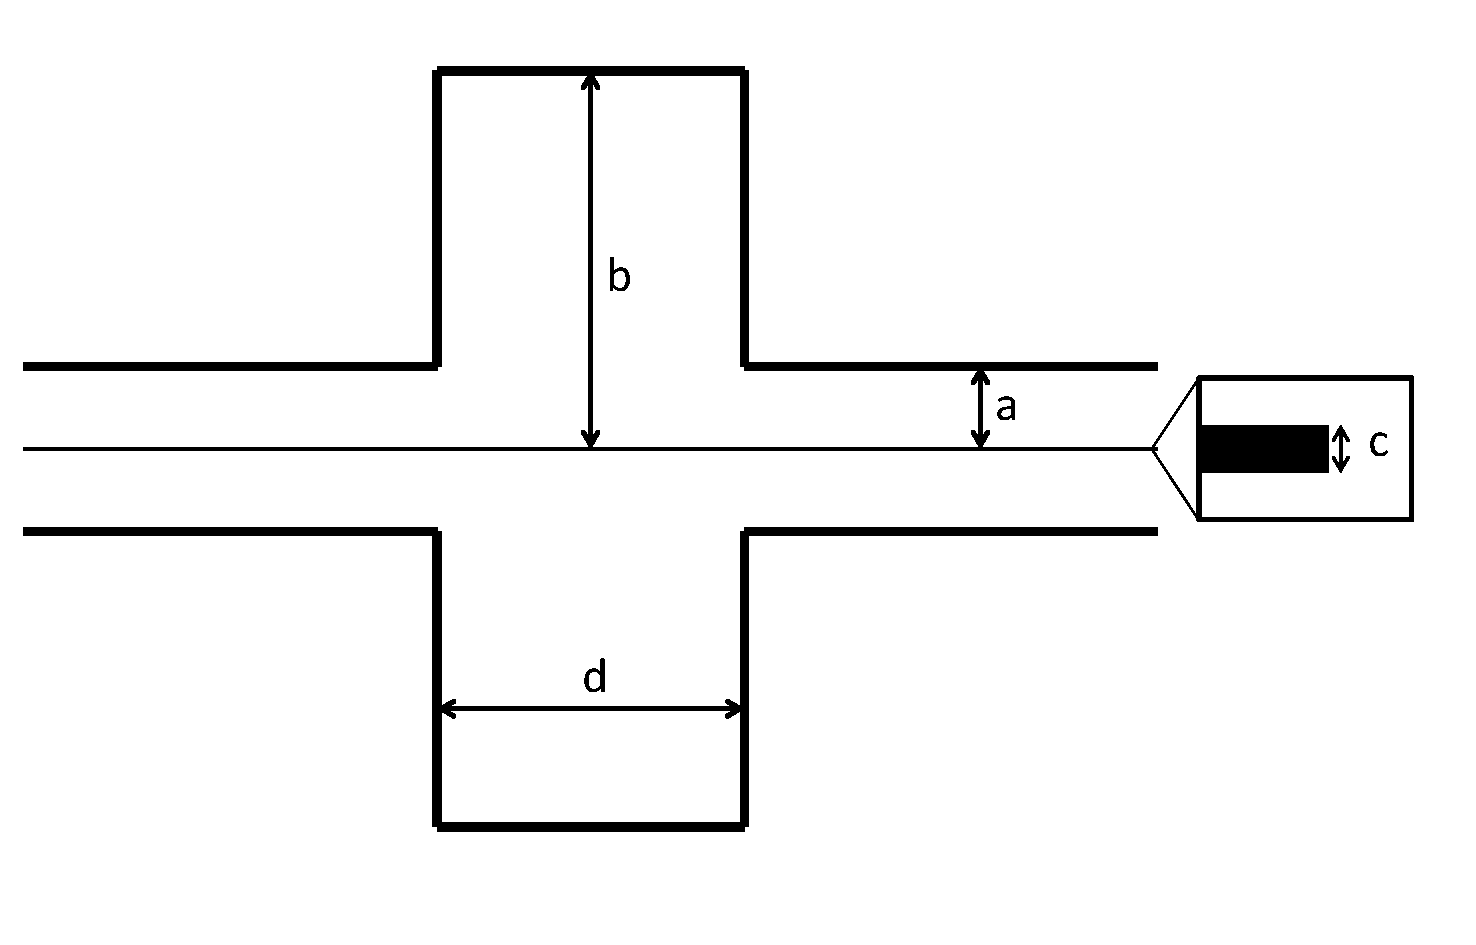
\includegraphics[width=0.625\linewidth]{figures/cavity_beampipe_coaxial.pdf}
\label{fig:cavity_beampipe_coaxial}
}
\caption{Comparison of the geometries of a cavity and attached beampipes \subref{fig:cavity_beampipe} without and \subref{fig:cavity_beampipe_coaxial} with the coaxial wire in place. Note the dimensions and that the dashed line in \subref{fig:cavity_beampipe} and the solid line in \subref{fig:cavity_beampipe_coaxial} represent the rotational plane of symmetry}
\end{figure}

\begin{figure}
\begin{center}
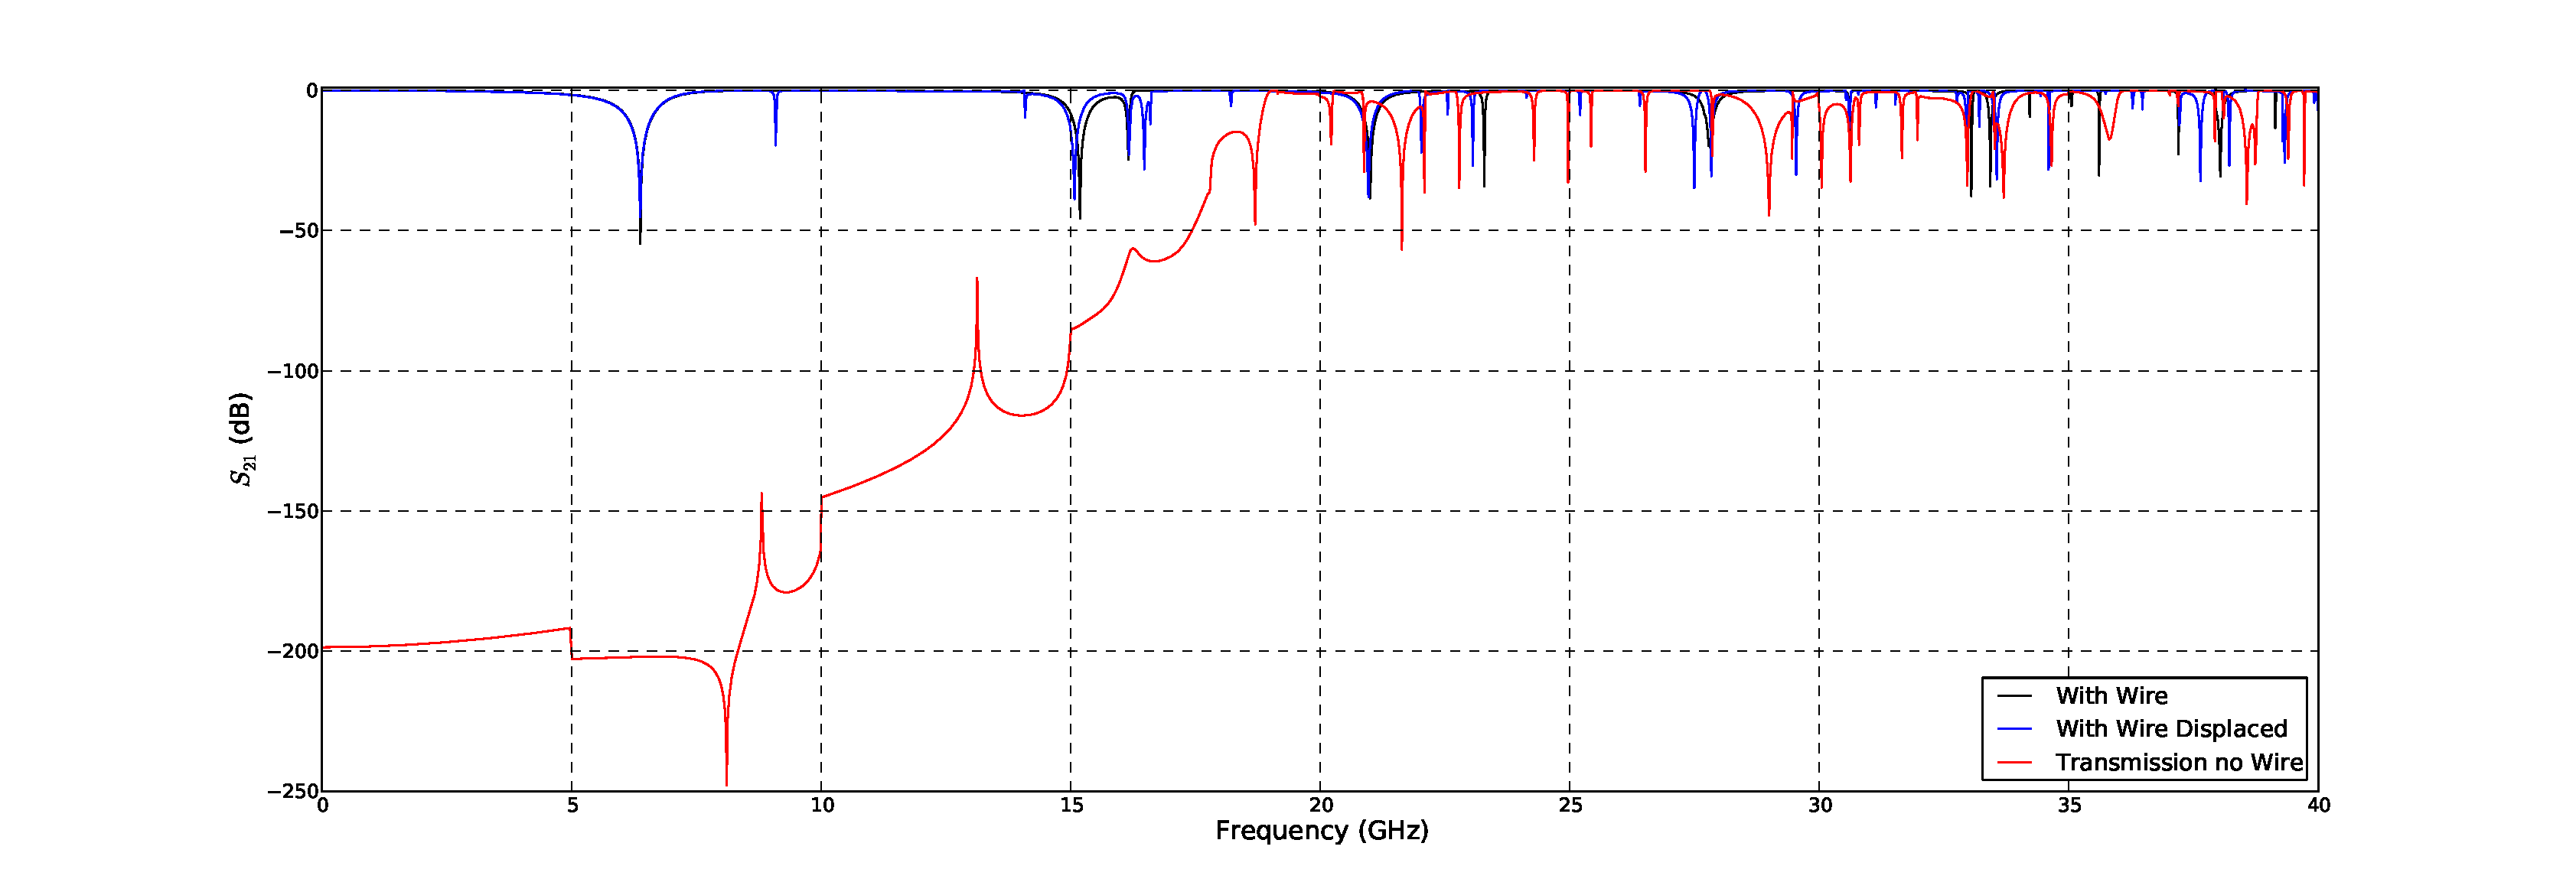
\includegraphics[width=1.1\textwidth]{Bench_Top_Measurements/figures/coax-trans-cavity.pdf}
\end{center}
\caption{A comparison of the transmission parameters through a pillbox cavity with and without a coaxial wire. A displaced coaxial wire is also shown to illustrate the possibility of exciting dipolar modes also. It can be seen that the transmission signals are drastically changed depending on the presence or not of the wire.}
\label{fig:cav-wire-tans}
\end{figure}

%
%  Things to do for high Q factor measurements
% - Simulation of transmission coefficients with and without coaxial wire
% - Comparison of impedance due to these resonances with time domain simulations
%
%
%
%
%
%
%
%
%
%
